%
% ---------------------------------------------------------------
% Copyright (C) 2012-2018 Gang Li
% ---------------------------------------------------------------
%
% This work is the default powerdot-tuliplab style test file and may be
% distributed and/or modified under the conditions of the LaTeX Project Public
% License, either version 1.3 of this license or (at your option) any later
% version. The latest version of this license is in
% http://www.latex-project.org/lppl.txt and version 1.3 or later is part of all
% distributions of LaTeX version 2003/12/01 or later.
%
% This work has the LPPL maintenance status "maintained".
%
% This Current Maintainer of this work is Gang Li.
%
%

\documentclass[
 size=14pt,
 paper=smartboard,  %a4paper, smartboard, screen
 mode=present, 		%present, handout, print
 display=slides, 	% slidesnotes, notes, slides
 style=tuliplab,  	% TULIP Lab style
 pauseslide,
 fleqn,leqno]{powerdot}{}

\usepackage{smartdiagram}
\usepackage{amssymb}
\usepackage{amsmath}
\usepackage{rotating}
\usepackage{graphicx}
\usepackage{boxedminipage}
\usepackage{media9}
\usepackage{rotate}
\usepackage{calc}
\usepackage[absolute]{textpos}
\usepackage{psfrag,overpic}
\usepackage{fouriernc}
\usepackage{pstricks,pst-node,pst-text,pst-3d,pst-grad}
\usepackage{moreverb,epsfig,subfigure}
\usepackage{pstricks}
\usepackage{pstricks-add}
\usepackage{pst-text}
\usepackage{pst-node, pst-tree}
\usepackage{booktabs}
\usepackage{etex}
\usepackage{breqn}
\usepackage{multirow}
\usepackage{gitinfo2}
\usepackage{xcolor}
\usepackage{multicol}
\usepackage{ulem}
\usepackage{todonotes}
\usepackage{tablefootnote}
\usepackage{threeparttable}
\usepackage[numbers]{natbib}
\usepackage{bibentry}
% \usepackage{pst-rel-points}
\usepackage{pgfplots}
\usepackage{verbatim}

\usepackage{listings}
\lstset{frameround=fttt,
frame=trBL,
stringstyle=\ttfamily,
backgroundcolor=\color{yellow!20},
basicstyle=\footnotesize\ttfamily}
\lstnewenvironment{code}{
\lstset{frame=single,escapeinside=`',
backgroundcolor=\color{yellow!20},
basicstyle=\footnotesize\ttfamily}
}{}


\usepackage{hyperref}
\hypersetup{ % TODO: PDF meta Data
  pdftitle={TULIP Lab},
  pdfauthor={Gang Li},
  pdfpagemode={FullScreen},
  pdfborder={0 0 0}
}


% \usepackage{auto-pst-pdf}
% package to show source code

%\definecolor{LightGray}{rgb}{0.9,0.9,0.9}
\definecolor{antiquebrass}{rgb}{0.8, 0.58, 0.46}
\newlength{\pixel}\setlength\pixel{0.000714285714\slidewidth}
\setlength{\TPHorizModule}{\slidewidth}
\setlength{\TPVertModule}{\slideheight}
\newcommand\highlight[1]{\fbox{#1}}
\newcommand\icite[1]{{\footnotesize [#1]}}

\newcommand\twotonebox[2]{\fcolorbox{pdcolor2}{pdcolor2}
{#1\vphantom{#2}}\fcolorbox{pdcolor2}{white}{#2\vphantom{#1}}}
\newcommand\twotoneboxo[2]{\fcolorbox{pdcolor2}{pdcolor2}
{#1}\fcolorbox{pdcolor2}{white}{#2}}
\newcommand\vpspace[1]{\vphantom{\vspace{#1}}}
\newcommand\hpspace[1]{\hphantom{\hspace{#1}}}
\newcommand\COMMENT[1]{}

\newcommand\placepos[3]{\hbox to\z@{\kern#1
        \raisebox{-#2}[\z@][\z@]{#3}\hss}\ignorespaces}

\renewcommand{\baselinestretch}{1.2}


\newcommand{\draftnote}[3]{
	\todo[author=#2,color=#1!30,size=\footnotesize]{\textsf{#3}}	}
% TODO: add yourself here:
%
\newcommand{\gangli}[1]{\draftnote{blue}{GLi:}{#1}}
\newcommand{\shaoni}[1]{\draftnote{green}{sn:}{#1}}
\newcommand{\mengren}[1]{\draftnote{orange}{MRen:}{#1}}
\newcommand{\xinhan}[1]{\draftnote{red}{Xhan:}{#1}}
\newcommand{\gliMarker}
	{\todo[author=GLi,size=\tiny,inline,color=blue!40]
	{Gang Li has worked up to here.}}
\newcommand{\snMarker}
	{\todo[author=Sn,size=\tiny,inline,color=green!40]
	{Shaoni has worked up to here.}}
\newcommand{\mrMarker}
	{\todo[author=MRen,size=\tiny,inline,color=orange!40]
	{Meng Ren has worked up to here.}}
\newcommand{\xhMarker}
	{\todo[author=XHan,size=\tiny,inline,color=red!40]
	{XinHan has worked up to here.}}
\newcommand{\zhMarker}
{\todo[author=ZHou,size=\tiny,inline,color=purple!40]
	{Ziwei Hou has worked up to here.}}

\usepackage{geometry}
\geometry{verbose,letterpaper}
\usepackage{movie15}
\usepackage{hyperref}

\usepackage[utf8]{inputenc}
\usepackage{dtk-logos}
\usepackage{tikz}
\usetikzlibrary{arrows,chains,mindmap,shadows,automata,patterns,petri,shapes.geometric,shapes.misc, spy, trees}
%\usepackage[hidelinks,pdfencoding=auto]{hyperref}
% Information boxes
\newcommand*{\info}[4][4]{%
  \node [ annotation, #3, text width = #1em,
          inner sep = 2mm ] at (#2) {%
  \list{$\bullet$}{\topsep=0pt\itemsep=0pt\parsep=0pt
    \parskip=0pt\labelwidth=2pt\leftmargin=2pt
    \itemindent=0pt\labelsep=2pt}%
    #4
  \endlist
  };
}

%forest
\usepackage{forest}
\usetikzlibrary{arrows.meta, shapes.geometric, calc, shadows}

\colorlet{mygreen}{green!75!black}
\colorlet{col1in}{red!30}
\colorlet{col1out}{red!40}
\colorlet{col2in}{mygreen!40}
\colorlet{col2out}{mygreen!50}
\colorlet{col3in}{blue!30}
\colorlet{col3out}{blue!40}
\colorlet{col4in}{mygreen!20}
\colorlet{col4out}{mygreen!30}
\colorlet{col5in}{blue!10}
\colorlet{col5out}{blue!20}
\colorlet{col6in}{blue!20}
\colorlet{col6out}{blue!30}
\colorlet{col7out}{orange}
\colorlet{col7in}{orange!50}
\colorlet{col8out}{orange!40}
\colorlet{col8in}{orange!20}
\colorlet{linecol}{blue!60}



%%%%%%%%%%%%%%%%%%%%%%%%%%%%%%%%%%%%%%%%%%%%%%%%%%%%%%%%%%%%%%%%%%%%%%%%
% title
% TODO: Customize to your Own Title, Name, Address
%
\title{Team for Universal Learning and Intelligent Processing}
\author{
Gang Li
\\
\\School of Information Technology
\\Deakin University, Australia
}
\date{\gitCommitterDate}


% Customize the setting of slides
\pdsetup{
% TODO: Customize the left footer, and right footer
rf=\href{http://www.tulip.org.au}{
Last Changed by: \textsc{\gitCommitterName}\ \gitVtagn-\gitAbbrevHash\ (\gitAuthorDate)
},
cf={TULIP Lab: Induction},
}


\begin{document}

\maketitle


%%==========================================================================================
%%
\begin{slide}[toc=,bm=]{Overview}
\tableofcontents[content=currentsection,type=1]
\end{slide}
%%
%%==========================================================================================


\section{TULIP Lab}
%%==========================================================================================
%%
\begin{slide}{Director}
  \twocolumn[lcolwidth=0.7\linewidth,
rcolwidth=0.3\linewidth
]{
    \begin{itemize}
      \item A/Prof. Gang Li
      \begin{itemize}
        \item \textcolor{orange}{IEEE Technical Committee}
         \begin{itemize}
           \item IEEE Task Force on EDM (Vice chair)
           \item Data Mining and Big Data Analytics (Vice Chair)
           \item Enterprise Architecture and Engineering
           \item Enterprise Information Systems
         \end{itemize}
        \item \textcolor{orange}{Deakin University}
          \begin{itemize}
            \item \emph{University Thesis Examination} Committee
            \item SEBE Faculty HDR Director
            \item Director for
                \begin{itemize}
                  \item \small{578/S678/S778/S779 (Master of Information Technology)}
                \end{itemize}
            \item Founding Director for
                \begin{itemize}
                  \item \small{S306 (Bachelor of Computer Science)}
                  \item \small{S777 (Master of Data Science)}
                \end{itemize}
          \end{itemize}
      \end{itemize}
    \end{itemize}}
    {\begin{flushleft}
       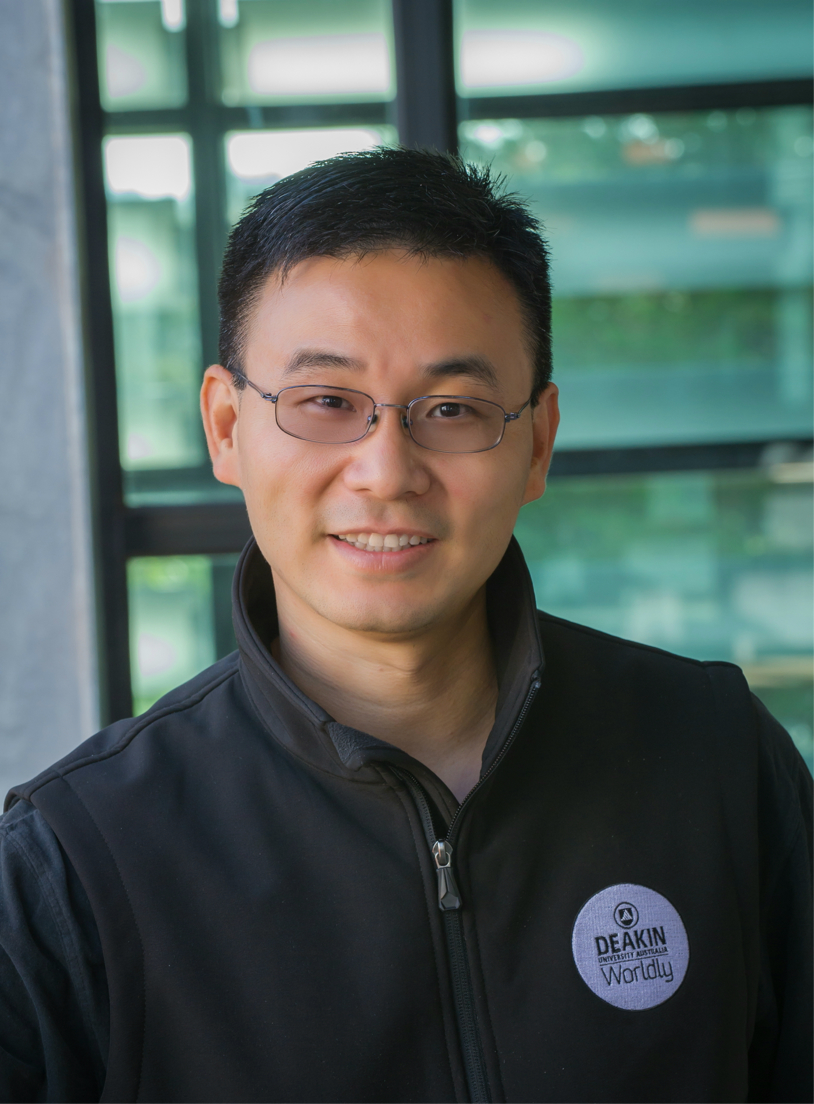
\includegraphics[width=0.8\textwidth]{figures//li//2014gangli.eps}
     \end{flushleft}
    }
\end{slide}
%%
%%===============================================================================

%%
%%===============================================================================
%\begin{slide}[toc=,bm=]{Director}
%\selectcolormodel{rgb}
%\begin{itemize}
%  \item A/Prof. Gang Li
%  \twocolumn[lcolwidth=0.5\linewidth,
%rcolwidth=0.5\linewidth
%]{\begin{center}
%\scalebox{0.65}{
%\smartdiagramset{distance center/other bubbles=1.5cm,}
%\smartdiagram[bubble diagram]{
%IEEE Technical \\ Committee,IEEE Task \\Force on EDM\\(Vice Chair) ,Data Mining \\and Big Data\\ Analytics\\(Vice Chair),Enterprise \\ Architecture\\and Engineering,Enterprise\\Information\\Systems%
%}}
%
%\end{center}}{\begin{center}
%\smartdiagramset{bubble center node size=5cm,distance center/other bubbles=1.5cm,}
%\scalebox{0.65}{
%
%\smartdiagram[bubble diagram]{
%Deakin, University Thesis\\ Examination\\ Committee,SEBE Faculty\\ HDR  Director,Current Director\\ for S578~/S678~/\\S778~/S779 ,Founding Director\\for S306~/\\ S777%
%}}
%\end{center}}
%\end{itemize}
%
%\end{slide}
%%
%%==========================================================================================


%%==========================================================================================
%%
\begin{slide}{Organization}
\selectcolormodel{rgb}
\twocolumn[
%lcolwidth=0.3\textwidth,
%rcolwidth=0.6\textwidth
lcolwidth=0.6\linewidth,
rcolwidth=0.4\linewidth
]{
\begin{itemize}
  \item TULIP Lab
  \begin{itemize}
    \item \textcolor{orange}{Academy:} all members
    \item \textcolor{orange}{Headquarter:} PhD and Postdoc in Melbourne
    \item \textcolor{orange}{Master:} all master students
    \item \textcolor{orange}{Trainee:} all trainee students
        \begin{itemize}
          \item FLIP (00)
          \item FLIP (01)
          \item \dots
          \item FLIP (05)
        \end{itemize}
    \item \textcolor{orange}{Visitor:} visiting members
    \item \textcolor{orange}{Web Team:} web site maintaining and promotion team
  \end{itemize}
\end{itemize}}
{
\begin{center}
\scalebox{0.50}{
\smartdiagramset{planet color=orange!60,
distance planet-satellite=5cm,planet text width=3cm,
}
\smartdiagram[connected constellation diagram]
{TULIP Lab,Master,Trainee,Visitor,Web\\Team,Academy,Headquarter}}
\end{center}
}
\end{slide}
%%
%%==========================================================================================


%%==========================================================================================
%%

\begin{slide}{Organization}
\selectcolormodel{rgb}
\pgfkeys{/forest,
  rect/.append style   = {rectangle, rounded corners = 2pt,
                         inner color = col6in, outer color = col6out},
  ellip/.append style  = {ellipse, inner color = col5in,
                          outer color = col5out},
  orect/.append style  = {rect, font = \sffamily\bfseries\LARGE,
                         text width = 325pt, text centered,
                         minimum height = 10pt, outer color = col7out,
                         inner color=col7in},
  oellip/.append style = {ellip, inner color = col8in, outer color = col8out,
                          font = \sffamily\bfseries\large, text centered}}
\begin{forest}
  for tree={
      font=\sffamily\bfseries,
      line width=1pt,
      draw=linecol,
      ellip,
      align=center,
      child anchor=north,
      parent anchor=south,
      drop shadow,
      l sep+=12.5pt,
      edge path={
        \noexpand\path[color=linecol, rounded corners=5pt,
          >={Stealth[length=10pt]}, line width=1pt, ->, \forestoption{edge}]
          (!u.parent anchor) -- +(0,-5pt) -|
          (.child anchor)\forestoption{edge label};
        },
      where level={3}{tier=tier3}{},
      where level={0}{l sep-=15pt}{},
      where level={1}{
        if n={1}{
          edge path={
            \noexpand\path[color=linecol, rounded corners=5pt,
              >={Stealth[length=10pt]}, line width=1pt, ->,
              \forestoption{edge}]
              (!u.west) -| (.child anchor)\forestoption{edge label};
            },
        }{
          edge path={
            \noexpand\path[color=linecol, rounded corners=5pt,
              >={Stealth[length=10pt]}, line width=1pt, ->,
              \forestoption{edge}]
              (!u.east) -| (.child anchor)\forestoption{edge label};
            },
        }
      }{},
  }
  [Academy, inner color=col1in, outer color=col1out
    [Web Team, inner color=col2in, outer color=col2out]
    [Trainee, inner color=col3in, outer color=col3out
      [Headquarter]
      [Master]
      [Visitor]
    ]
    [Alumni, inner color =col7in, outer color = col7out ]
  ]
\end{forest}
\end{slide}
%%
%%==========================================================================================


%%==========================================================================================
%%
\begin{slide}{Deakin Rankings}
\begin{table}[htbp]
  \setlength{\abovecaptionskip}{-2pt}
  \setlength{\belowcaptionskip}{12pt}
  \centering
%  \caption{Deakin Ranking in Major Ranking}
    \begin{tabular}{l|c|cccr}
    \toprule
      & Benchmark & \multicolumn{1}{l}{2014-15} & \multicolumn{1}{l}{2015-2016} & \multicolumn{1}{l}{2016-2017} & \multicolumn{1}{l}{2017-2018} \\ \midrule
    \multirow{2}[0]{*}{ARWU} & World & 401-500 & 301-400 & 201-300 & 201 \\
      & National  & 19 &   &   & 10 \\
      \midrule
    \multirow{2}[0]{*}{CWTS Leiden} & World  & 284 & 325 & 314 & 226 \\
      & National  & 11 & 17 & 17 & 11 \\
      \midrule
    \multirow{2}[0]{*}{QS\#} & World  & 360 & 324 & 355 & 293 \\
      & National & 19 &   &   &  \\
      \midrule
    \multirow{2}[0]{*}{THE} & World  & 325 & 301-350 & 251-300 & 301 \\
      & National  & 13 &   &   & 17 \\
      \midrule
    \multirow{2}[0]{*}{THE<50} & World  & 59 &   &   & 43 \\
      & National  & 7 &   &   & 8 \\
      \bottomrule
    \end{tabular}
  \label{tab:Deakin Ranking}
\end{table}
\centering
\url{https://www.australianuniversities.com.au/rankings/}
\end{slide}
%%
%%==========================================================================================


%%==========================================================================================
%%
%\begin{slide}{TULIP Lab}
%
%\begin{itemize}
%  \item \textcolor{orange}{Homepage:} \href{https://weibo.com/tulipacademy}{https://weibo.com/tulipacademy}
%  \begin{itemize}
%    \item Twitter: tulipacademy
%    \item Weibo: \href{https://weibo.com/tulipacademy}{https://weibo.com/tulipacademy}
%  \end{itemize}
%  \item \textcolor{orange}{Github:} \href{https://github.com/tulip-lab}{https://github.com/tulip-lab}
%  \item \textcolor{orange}{Tulip Calendar:}
%  \begin{itemize}
%    \item\href{https://calendar.google.com/calendar/embed?src=1trnk46p4gae8ev410ku57sba4\%40group.calendar.google.com\&ctz=Australia\%2FSydney
%}{https://calendar.google.com/calendar/embed?src=1trnk46p4gae8ev410ku57sba4\%40group.calendar.google.com\&ctz=Australia\%2FSydney
%}
%    \item\href{https://calendar.google.com/calendar/ical/1trnk46p4gae8ev410ku57sba4\%40group.calendar.google.com/public/basic.ics
%}{https://calendar.google.com/calendar/ical/1trnk46p4gae8ev410ku57sba4\%40group.calendar.google.com/public/basic.ics
%}
%  \end{itemize}
%\end{itemize}
%
%\end{slide}
%%
%%==========================================================================================


\section{Research @ TULIP}


%%==========================================================================================
%%
\begin{slide}[toc=,bm=]{Research Themes}
\begin{center}

\selectcolormodel{rgb}
   \begin{tikzpicture}[ every annotation/.style = {draw,
                     fill = white}]
  \path[mindmap,concept color=blue!50,text=white,
    every node/.style={concept},
    root/.style    = {concept color=black!40,
      font=\Large\bfseries,text width=10em},
    level 1 concept/.append style={font=\bfseries,
      sibling angle=100,text width=7.7em,level distance=8em,inner sep=0pt},
    level 2 concept/.append style={font=\sf,sibling angle=80,text width=7em,inner sep=0pt},
  ]
  node[root,scale=0.6,concept color=blue!50, text=white] {Research Themes} [clockwise from=180]
    child[concept color=orange!60] {
      node[scale=0.6] {Behavior Informatics} [clockwise from=200]
        child { node[scale=0.6] (pbm){Periodic Behavior Mining}}
        child { node[scale=0.6] (bp) {Behavior Prediction}}
    }
     child[concept color=blue!60] {
      node[concept,scale=0.6] {Data Privacy}[clockwise from=120]
      child{node[concept,scale=0.6](dcc){Data Compliance Checking}}
      child{node[concept,scale=0.6](privacy){Privacy Preservation in Data Mining}}
    }
    child[concept color=blue!60] {
      node[concept,scale=0.6] {Business Intelligence Application}[clockwise from=60]
      child{node[concept,scale=0.6](rs){Recommender System} }
      child{node[concept,scale=0.6](t/hm){Tourism / Hospitality Management}}
    }
   ;
    \end{tikzpicture}
\end{center}
%%==========================================================================================
\begin{note}
Behavior Informatics: Periodic Behavior Mining, Behavior Prediction\\
Information Abuse Prevention: Data Compliance Checking, Privacy Preservation in Data Mining\\
Business Intelligence Applications: Recommender System, Tourism/Hospitality Management
\end{note}
%%==========================================================================================
\end{slide}
%%
%%==========================================================================================


%%==========================================================================================
%%
\begin{slide}{Research Themes}
\begin{center}

\selectcolormodel{rgb}
   \begin{tikzpicture}[ every annotation/.style = {draw,
                     fill = white}]
  \path[mindmap,concept color=blue!50,text=white,
    every node/.style={concept},
    root/.style    = {concept color=black!40,
      font=\Large\bfseries,text width=10em},
    level 1 concept/.append style={font=\bfseries,
      sibling angle=100,text width=7.7em,level distance=8em,inner sep=0pt},
    level 2 concept/.append style={font=\sf,sibling angle=80,text width=7em,inner sep=0pt},
  ]
  node[root,scale=0.6,concept color=blue!50, text=white] {Research Themes} [clockwise from=180]
    child[concept color=blue!60] {
      node[scale=0.6] {Behavior Informatics} [clockwise from=200]
        child { node[scale=0.6] (pbm){Periodic Behavior Mining}}
        child { node[scale=0.6] (bp) {Behavior Prediction}}
    }
     child[concept color=orange!60] {
      node[concept,scale=0.6] {Data Privacy}[clockwise from=120]
      child{node[concept,scale=0.6](dcc){Data Compliance Checking}}
      child{node[concept,scale=0.6](privacy){Privacy Preservation in Data Mining}}
    }
    child[concept color=blue!60] {
      node[concept,scale=0.6] {Business Intelligence Application}[clockwise from=60]
      child{node[concept,scale=0.6](rs){Recommender System} }
      child{node[concept,scale=0.6](t/hm){Tourism / Hospitality Management}}
    }
   ;
    \end{tikzpicture}
\end{center}

\end{slide}
%%
%%==========================================================================================

%%==========================================================================================
%%
\begin{slide}{Research Themes}
\begin{center}

\selectcolormodel{rgb}
   \begin{tikzpicture}[ every annotation/.style = {draw,
                     fill = white}]
  \path[mindmap,concept color=blue!50,text=white,
    every node/.style={concept},
    root/.style    = {concept color=black!40,
      font=\Large\bfseries,text width=10em},
    level 1 concept/.append style={font=\bfseries,
      sibling angle=100,text width=7.7em,level distance=8em,inner sep=0pt},
    level 2 concept/.append style={font=\sf,sibling angle=80,text width=7em,inner sep=0pt},
  ]
  node[root,scale=0.6,concept color=blue!50, text=white] {Research Themes} [clockwise from=180]
    child[concept color=blue!60] {
      node[scale=0.6] {Behavior Informatics} [clockwise from=200]
        child { node[scale=0.6] (pbm){Periodic Behavior Mining}}
        child { node[scale=0.6] (bp) {Behavior Prediction}}
    }
     child[concept color=blue!60] {
      node[concept,scale=0.6] {Data Privacy}[clockwise from=120]
      child{node[concept,scale=0.6](dcc){Data Compliance Checking}}
      child{node[concept,scale=0.6](privacy){Privacy Preservation in Data Mining}}
    }
    child[concept color=orange!60] {
      node[concept,scale=0.6] {Business Intelligence Application}[clockwise from=60]
      child{node[concept,scale=0.6](rs){Recommender System} }
      child{node[concept,scale=0.6](t/hm){Tourism / Hospitality Management}}
    }
   ;
    \end{tikzpicture}
\end{center}

\end{slide}
%%
%%==========================================================================================

%%==========================================================================================
%%
%\begin{slide}{Theme 1. Behavior Informatics}
%%Theme one -
%\begin{itemize}
%\item
%People share \textcolor{blue!50}{news, interests}
%and \textcolor{blue!50}{ideas} in OSNs
%
%\begin{itemize}
%\item
%\textbf{though} these platforms also spread
%\textcolor{orange}{email malware, rumours, gossips}
%\textcolor{orange}{and malicious links}, and may even leak our
%\textcolor{orange}{privacy}.
%\end{itemize}
%\end{itemize}
%
%\twocolumn{
%\begin{figure}[htbp]
%  %  \centering
%    \subfigure{
%        
\includegraphics[width=0.28\textwidth]{figures//theme1//Theme1_1.eps}
%    }
%    \subfigure{
%        
\includegraphics[width=0.28\textwidth]{figures//theme1//Theme1_2.eps}
%    }
%    \subfigure{
%        
\includegraphics[width=0.28\textwidth]{figures//theme1//Theme1_3.eps}
%    }\\
%    \subfigure{
%        
\includegraphics[width=0.28\textwidth]{figures//theme1//Theme1_4.eps}
%    }
%    \subfigure{
%        
\includegraphics[width=0.28\textwidth]{figures//theme1//Theme1_5.eps}
%    }
%    \subfigure{
%        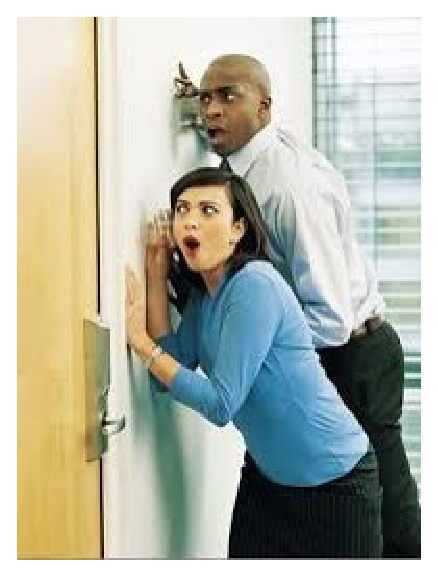
\includegraphics[width=0.28\textwidth]{figures//theme1//Theme1_6.eps}
%    }
%\end{figure}
%}{
%\begin{figure}[htbp]
%    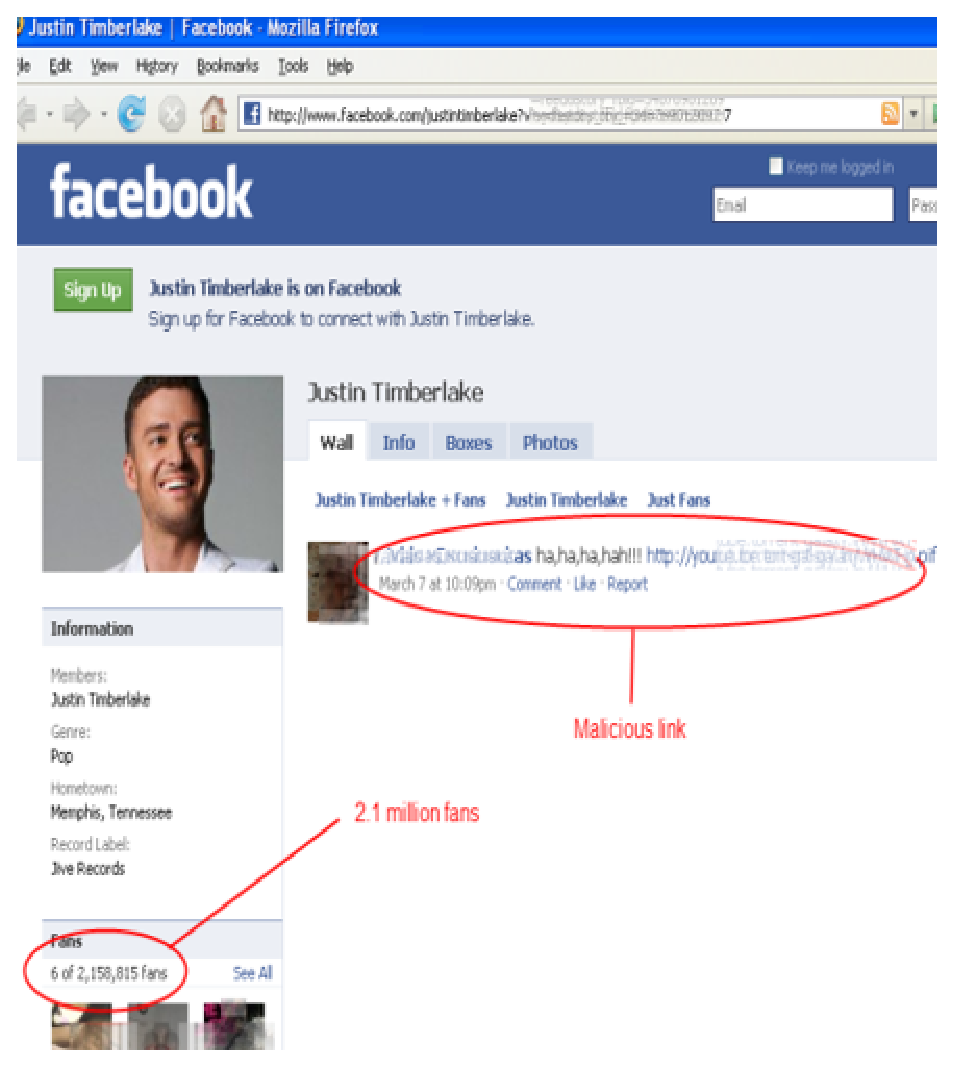
\includegraphics[width=0.7\textwidth]{figures//theme1//Theme1_7.eps}
%\end{figure}
%}
%
%\end{slide}
%%
%%==========================================================================================


%%==========================================================================================
%%
%\begin{slide}[toc=,bm=]{Theme 1. Behavior Informatics}
%
%\begin{itemize}
%\item
%The popularity of OSNs has greatly increased in recent years
%
%\begin{itemize}
%\item
%A large amount of Internet users also use OSN services
%
%\item
%Australia has up to $11$ million Facebook users
%\end{itemize}
%
%\end{itemize}
%
%\begin{figure}[htbp]
%    \centering
%    \subfigure{
%        
\includegraphics[width=0.25\textwidth]{figures//theme1//Theme1_8.eps}
%    }
%    \subfigure{
%        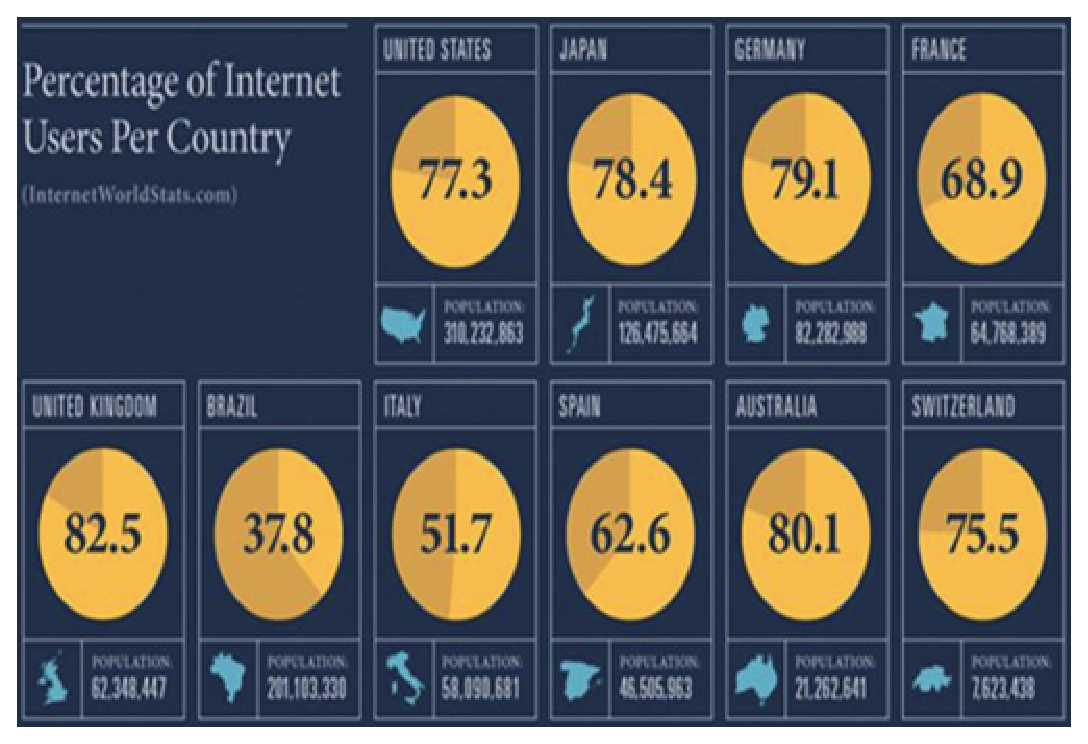
\includegraphics[width=0.37\textwidth]{figures//theme1//Theme1_9.eps}
%    }
%    \subfigure{
%        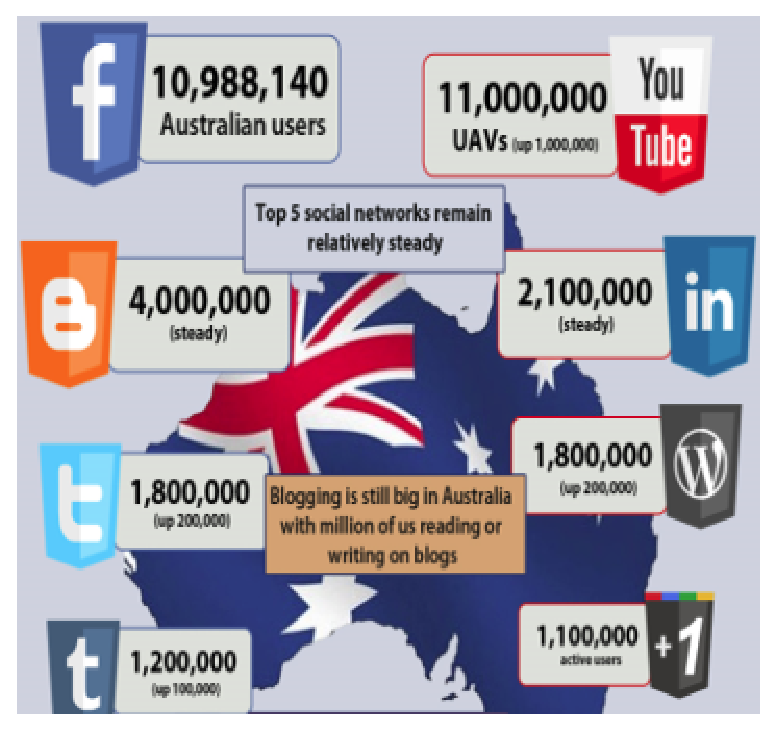
\includegraphics[width=0.3\textwidth]{figures//theme1//Theme1_10.eps}
%    }
%\end{figure}
%
%\end{slide}
%%
%%==========================================================================================


%%==========================================================================================
%%
\begin{slide}[toc=,bm=]{Case Study (1) - Tourist Movement Analysis}

\begin{itemize}
\item
There are many geotagged photos available.
However:

\begin{itemize}
\item
Data can be noisy or misleading

\item
Photos are taken in transit rather than at the attractions

\item
Photos are static media; whereas, travel behavior is dynamic
\end{itemize}

\end{itemize}
\begin{figure}[htbp]
    \centering
    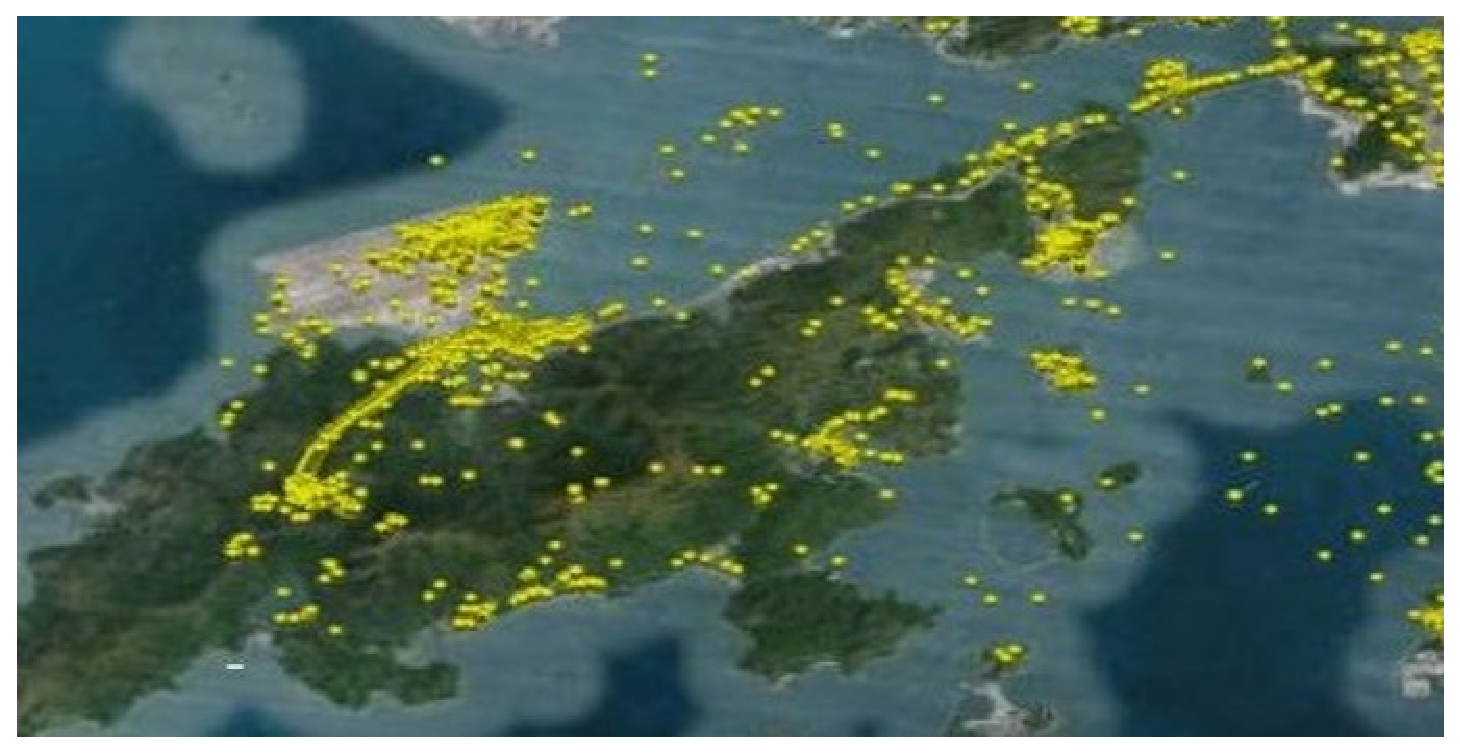
\includegraphics[width=0.5\textwidth]{figures//theme1//Theme1_11.eps}
\end{figure}

\begin{center}
   \onslide{2}{\twotonebox{\huge \textcolor{orange}{?}}
   {\large {How to mine these data for travel behaviour analysis?}}}
\end{center}

\end{slide}
%%
%%==========================================================================================


%%==========================================================================================
%%
\begin{slide}[toc=,bm=]{Case Study (1) - Tourist Movement Analysis}

\begin{itemize}
  \item Tourist Traffic Flow in Hong Kong Metropolitan Area
\end{itemize}

%\hspace{10}
\begin{figure}[htbp]
    \subfigure[Asian Tourist]{
        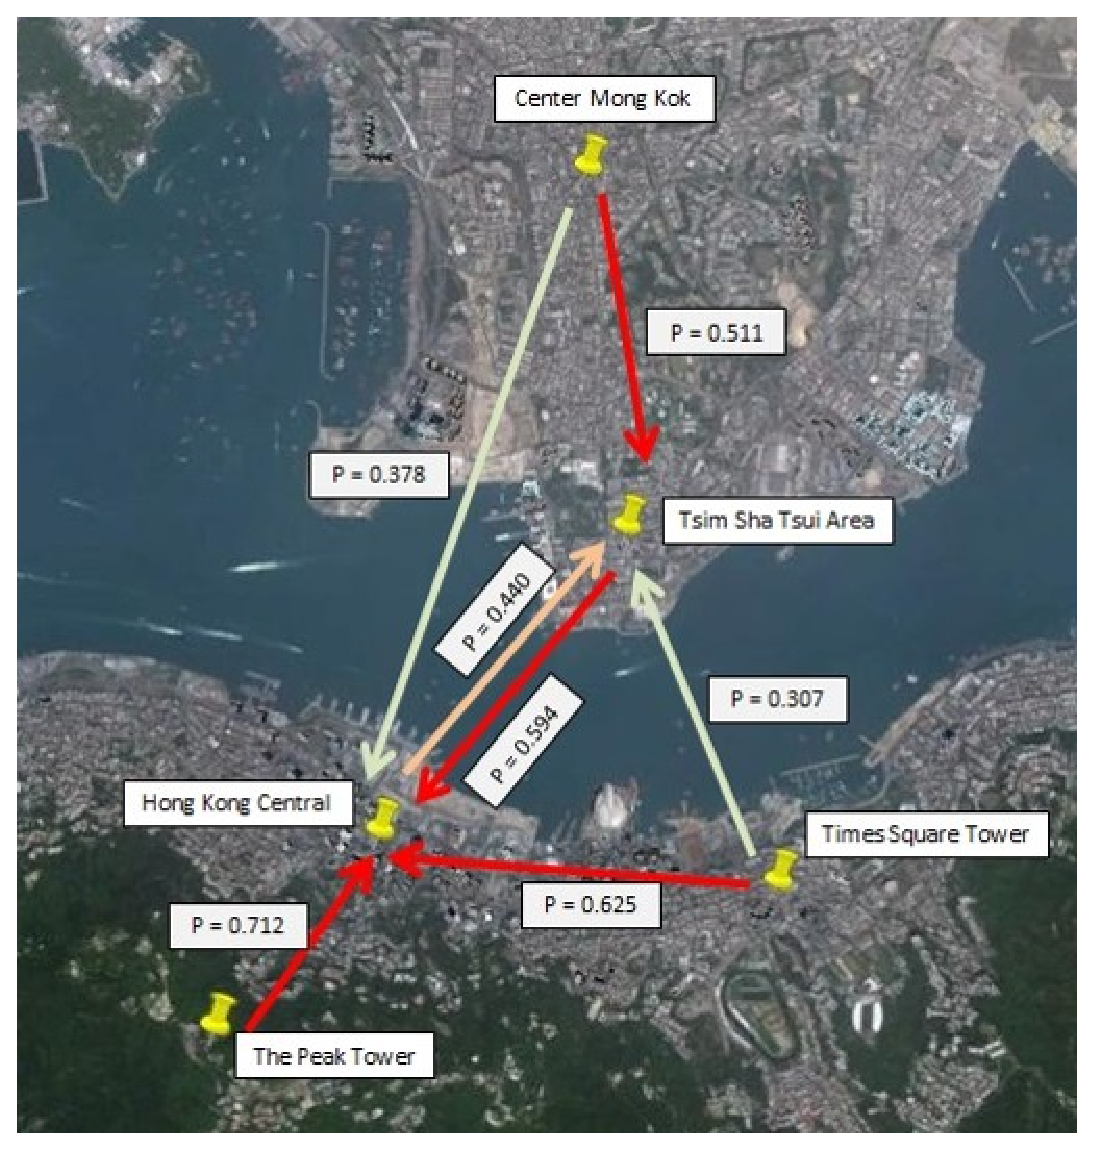
\includegraphics[width=0.3\textwidth]{figures//theme1//Theme1_12.eps}
    }
    \subfigure[Western Tourist]{
        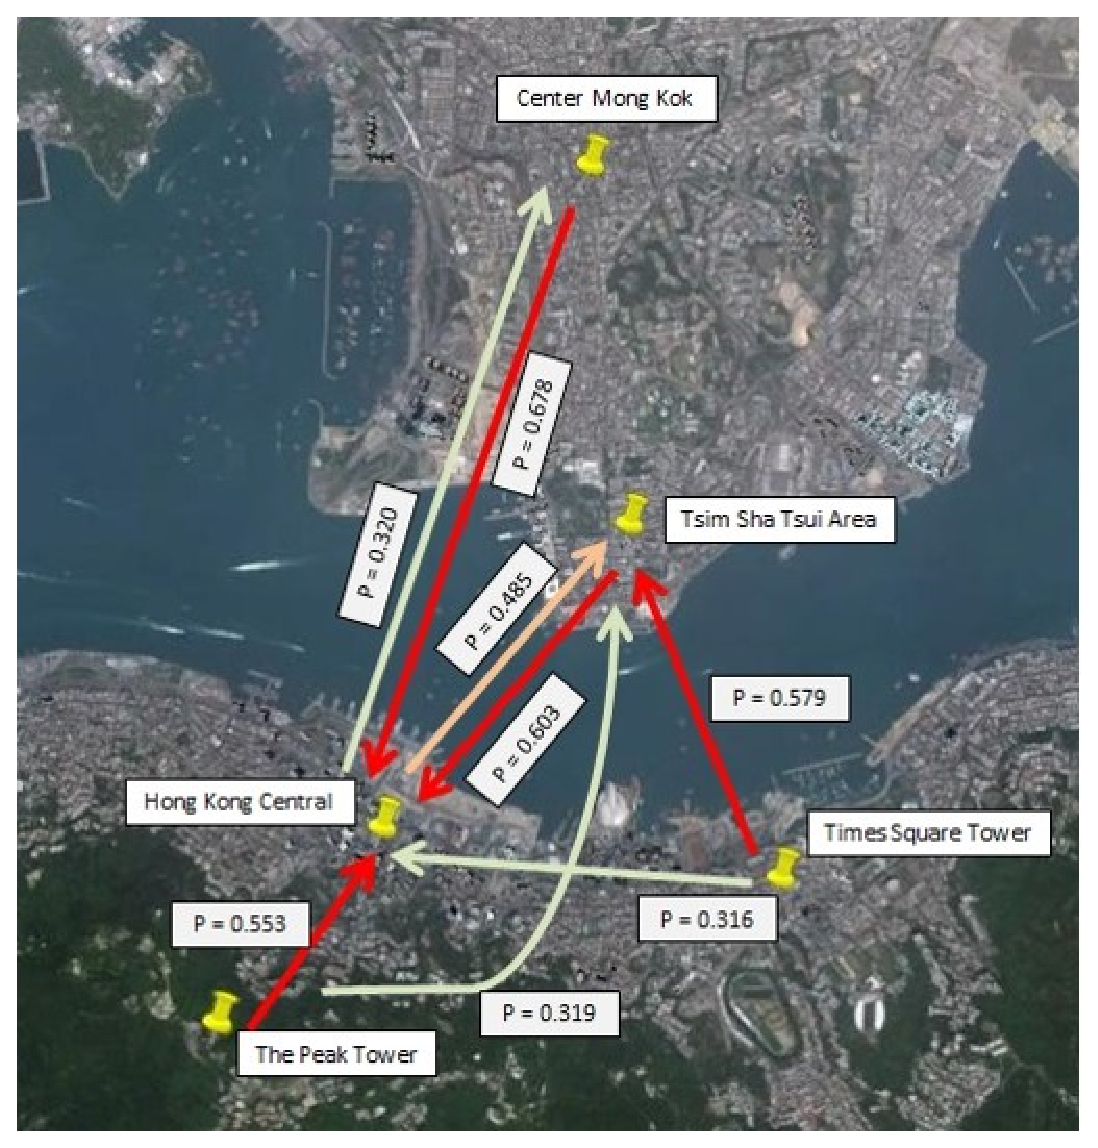
\includegraphics[width=0.3\textwidth]{figures//theme1//Theme1_13.eps}
    }
\end{figure}

\bibliographystyle{plain}
\nobibliography{tuliplab}
\footnotesize\bibentry{VLLY15J07}

\end{slide}
%%
%%==========================================================================================


%%==========================================================================================
%%
%\begin{slide}[toc=,bm=]{Case Study (2) - Periodic Behavior Mining}
%
%\begin{itemize}
%\item
%Observed check-in Data is usually a mixed event with different periodic behaviors
%
%\vspace{1cm}
%\twocolumn[lcolwidth=0.55\linewidth,
%rcolwidth=0.45\linewidth
%]{
%\begin{itemize}
%\item
%What is periodic behavior?
%
%\item
%What is the period of that behavior?
%
%\item
%Predict the behavior of a person on a particular day.
%\end{itemize}}
%{
%\begin{figure}[htbp]
%    \centering
%    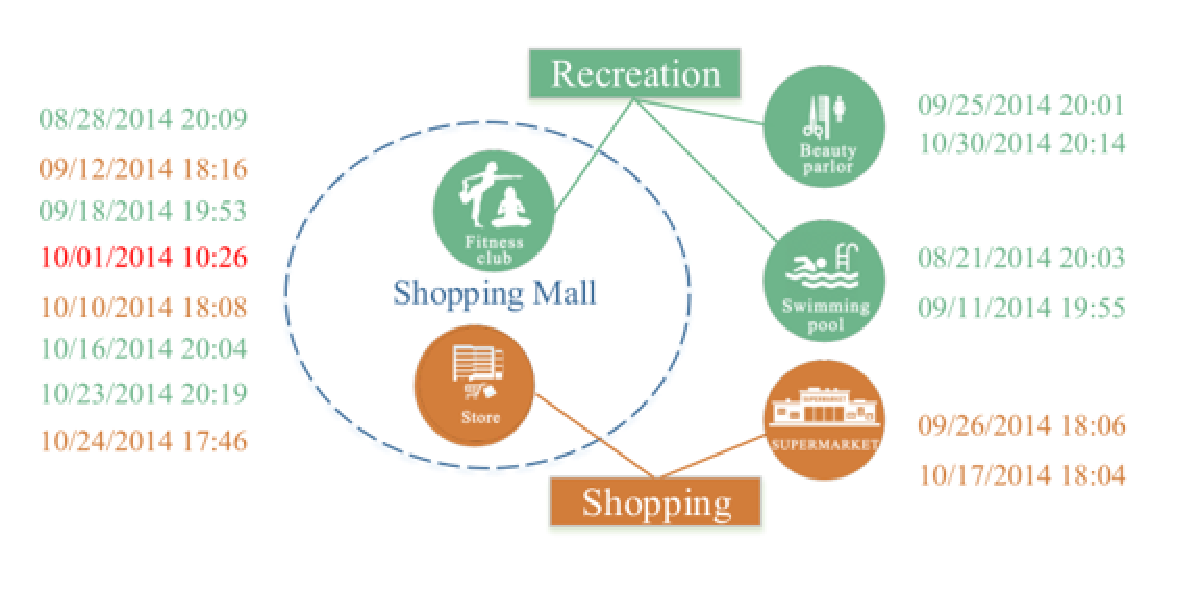
\includegraphics[width=0.9\textwidth]{figures//theme1//Theme1_18.eps}
%\end{figure}
%}
%
%\onslide*{2, 2-}{
%\begin{figure}[htbp]
%    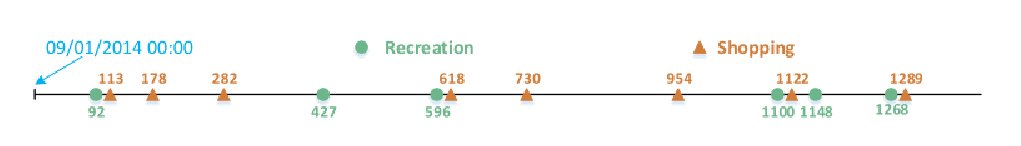
\includegraphics[width=0.7\textwidth]{figures//theme1//pbm_1.eps}
%\end{figure}
%}
%
%\onslide*{3, 3-}{
%\begin{figure}[htbp]
%    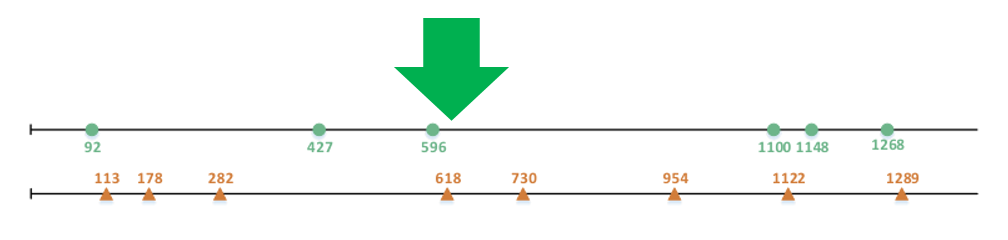
\includegraphics[width=0.7\textwidth]{figures//theme1//pbm_2.eps}
%\end{figure}
%}
%\end{itemize}
%
%\end{slide}
%%
%%==========================================================================================


%%==========================================================================================
%%
%\begin{slide}[toc=,bm=]{Case Study (2) - Periodic Behavior Mining}
%
%\begin{itemize}
%\item
%CP Decomposition
%\end{itemize}
%\vspace{0.5cm}
%\twocolumn{
%\begin{figure}[htbp]
%    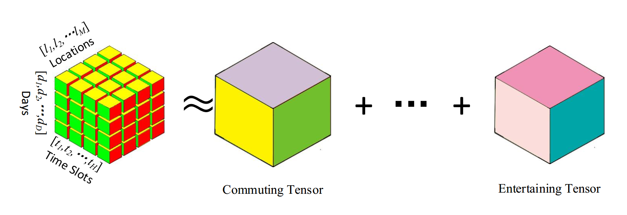
\includegraphics[width=0.8\textwidth]{figures//theme1//cpd_1.eps}
%\end{figure}
%}{
%\begin{flushleft}
%\large{
%$y_{r_i, t_j, d_k} = \frac{Count(r_i, t_j, d_k)}{\sum_{q=1}^L Count(r_q, t_j, d_k)}$
%}
%\end{flushleft}
%}
%
%\onslide*{2, 2-}{
%%\begin{center}
%\begin{figure}[htbp]
%    \subfigure{
%    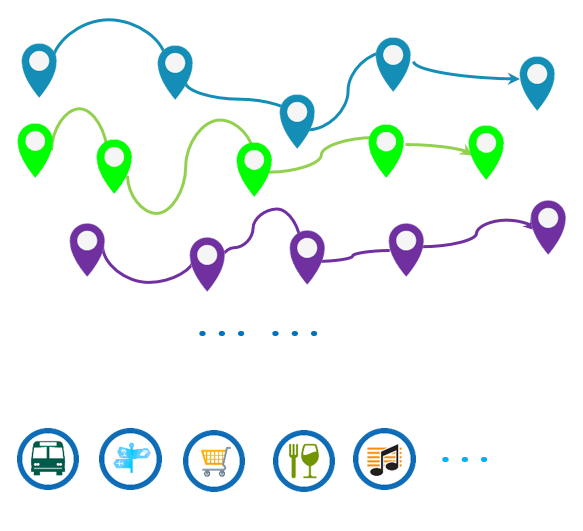
\includegraphics[width=0.29\textwidth]{figures//theme1//pbm_6.eps}
%    }
%    \subfigure{
%    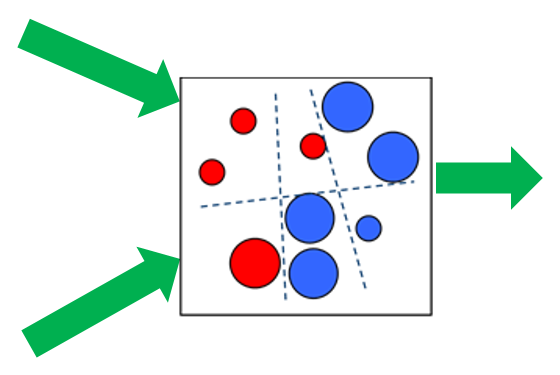
\includegraphics[width=0.32\textwidth]{figures//theme1//cpd_2.eps}
%    }
%    \subfigure{
%    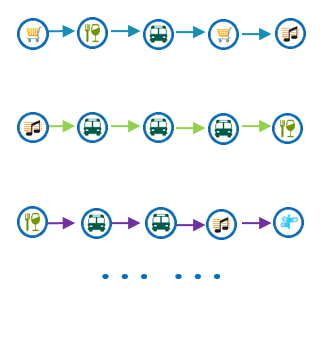
\includegraphics[width=0.2\textwidth]{figures//theme1//pbm_7.eps}
%    }
%\end{figure}
%%\end{center}
%}
%\end{slide}
%%
%%==========================================================================================


%%==========================================================================================
%%
\begin{slide}[toc=,bm=]{Case Study (2) - Periodic Behavior Mining}

\begin{itemize}
\item
There are various applications of \emph{Periodic Behavior Mining}

    \begin{itemize}
    \item
    What is the schedule of a person on a particular day or at a specified time?

    \item
    Where to find the person on a particular day or at a specified time?
        \begin{itemize}
        \item
        Police applications

        \item
        Scheduled ``Encountering'' for match making
        \end{itemize}
    \item
    Timely Recommendation Systems
        \begin{itemize}
        \item
        Recommend right before  the time for you to stock rice, cooking oil, or ice cream!
        \end{itemize}

\end{itemize}
\end{itemize}

\end{slide}
%%
%%==========================================================================================


%%==========================================================================================
%%
%\begin{slide}[toc=,bm=]{Case Study (3) - Face Age Recognition}
%
%\begin{figure}[htbp]
%    \subfigure{
%        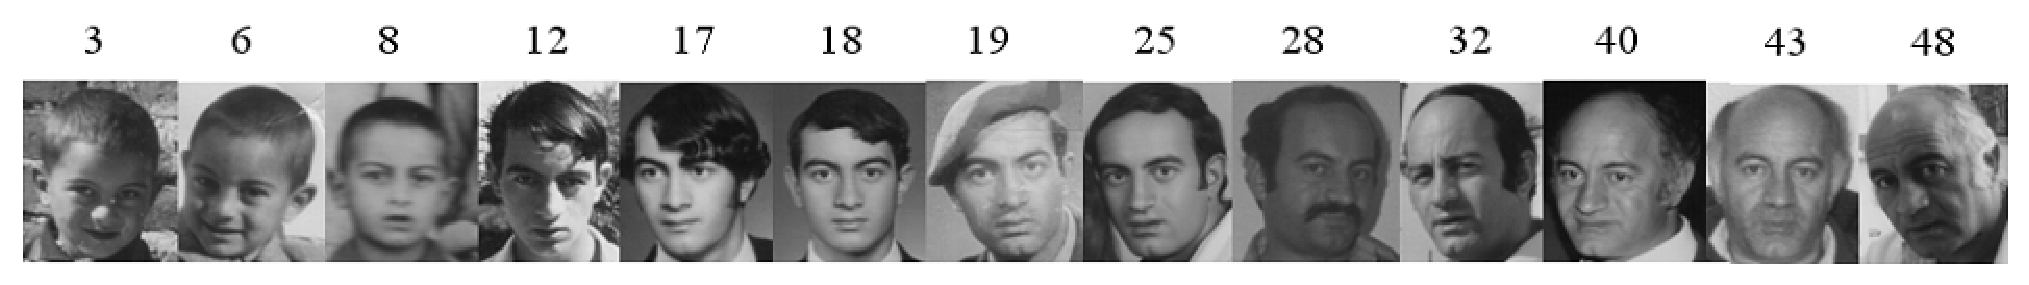
\includegraphics[width=0.8\textwidth]{figures//theme1//Theme1_19.eps}
%    }\\
%    \subfigure{
%        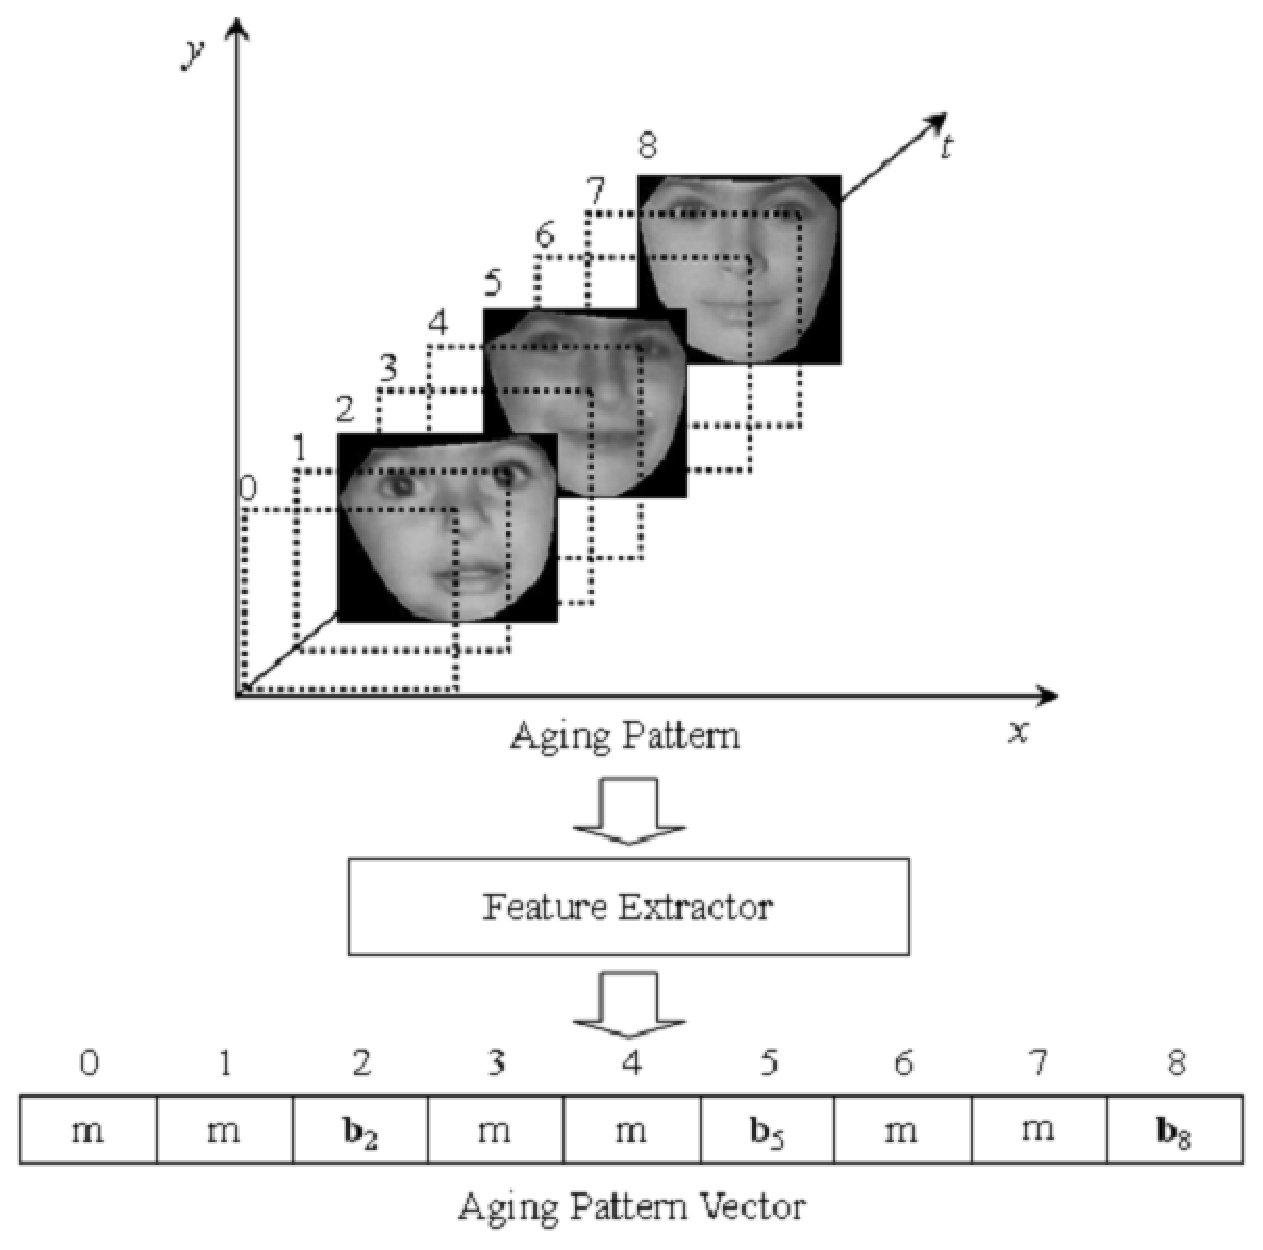
\includegraphics[width=0.3\textwidth]{figures//theme1//Theme1_20.eps}
%    }
%    \subfigure{
%        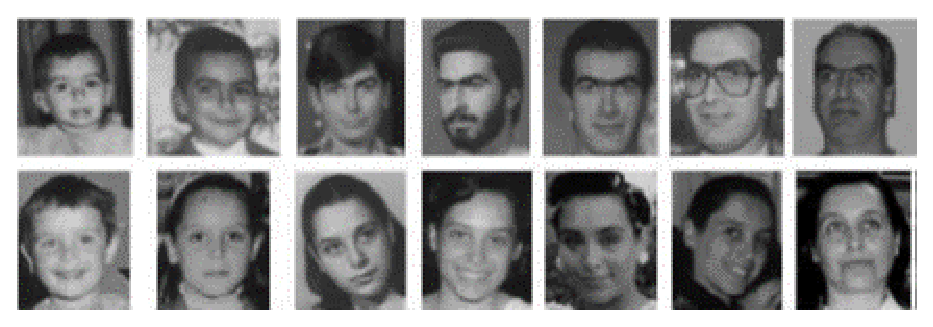
\includegraphics[width=0.4\textwidth]{figures//theme1//Theme1_21.eps}
%    }
%\end{figure}
%
%\bibliographystyle{plain}
%\nobibliography{tuliplab}
%\footnotesize\bibentry{GZZLD06C04}
%
%\end{slide}
%%
%%==========================================================================================


%%==========================================================================================
%%
\begin{slide}[toc=,bm=]{Case Study (4) - Speech Based Emotion Detection}

\begin{figure}
  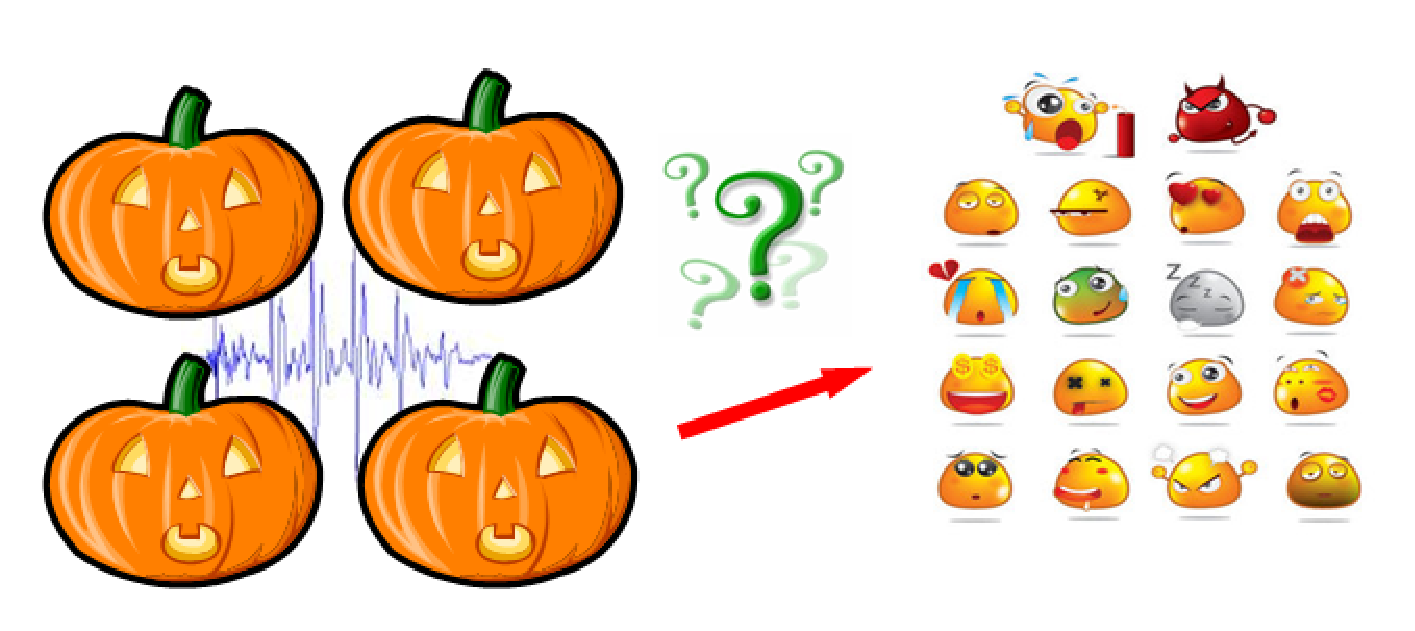
\includegraphics[width=0.8\textwidth]{figures//theme1//Theme1_22.eps}
\end{figure}

\bibliographystyle{plain}
\nobibliography{tuliplab}
\footnotesize\bibentry{RLC09J02}

\end{slide}
%%
%%==========================================================================================


%%==========================================================================================
%%
\begin{slide}[toc=,bm=]{Case Study (5) - K Complex Detection}
\begin{itemize}
\item Sleep Stage Identification
\begin{itemize}
\item<2->
\small{Rapid Eye Movement (REM) Sleep}
\begin{itemize}
\item<2->
\small{A normal stage of sleep characterized by the rapid movement of the eyes)}
\item<2->
\small{$20\%-25\%$ of total sleep time in human adults, memorable dream}
\end{itemize}
\item<3->
{Non-REM Sleep}
\begin{itemize}
\item<3->
\small{\textbf{$N_1$}: slow eye movement, hypnic jerks at beginning, believe fully awake}
\item<3->
\small{\textbf{$N_2$}: non eye movement, rare dreaming, easily awaken}
\item<3->
\small{\textbf{$N_3$}: deep sleep, sometimes dreaming, but disconnected, less vivid}
%\end{itemize}

\begin{figure}
  \begin{flushleft}
  % Requires \usepackage{graphicx}
  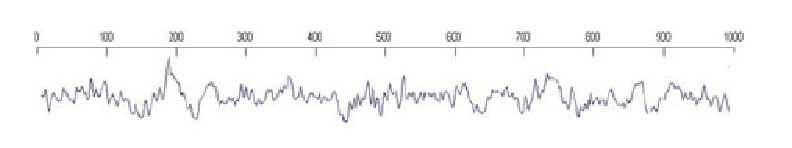
\includegraphics[width=0.4\textwidth]{figures//theme1//kcd.eps}
  \end{flushleft}
\end{figure}
\end{itemize}

\item<4->
General sleep order in cycles of REM and NREM:
$N_1 \rightarrow N_2 \rightarrow N_3 \rightarrow N_2 \rightarrow REM$
\begin{itemize}
\item<4->
\small{Early in the night, a greater amount of deep sleep (N3)}
\item<4->
\small{Later in the night, REM sleep increases, and before natural awakening}
\end{itemize}
\end{itemize}
\end{itemize}

\onslide*{4}
\bibliographystyle{plain}
\nobibliography{tuliplab}
\footnotesize\bibentry{VLSBLPAU12J03}

\end{slide}
%%
%%==========================================================================================


%%==========================================================================================
%%
\begin{slide}[toc=,bm=]{Case Study (6) - Trajectory Analysis}
\begin{figure}[htbp]
  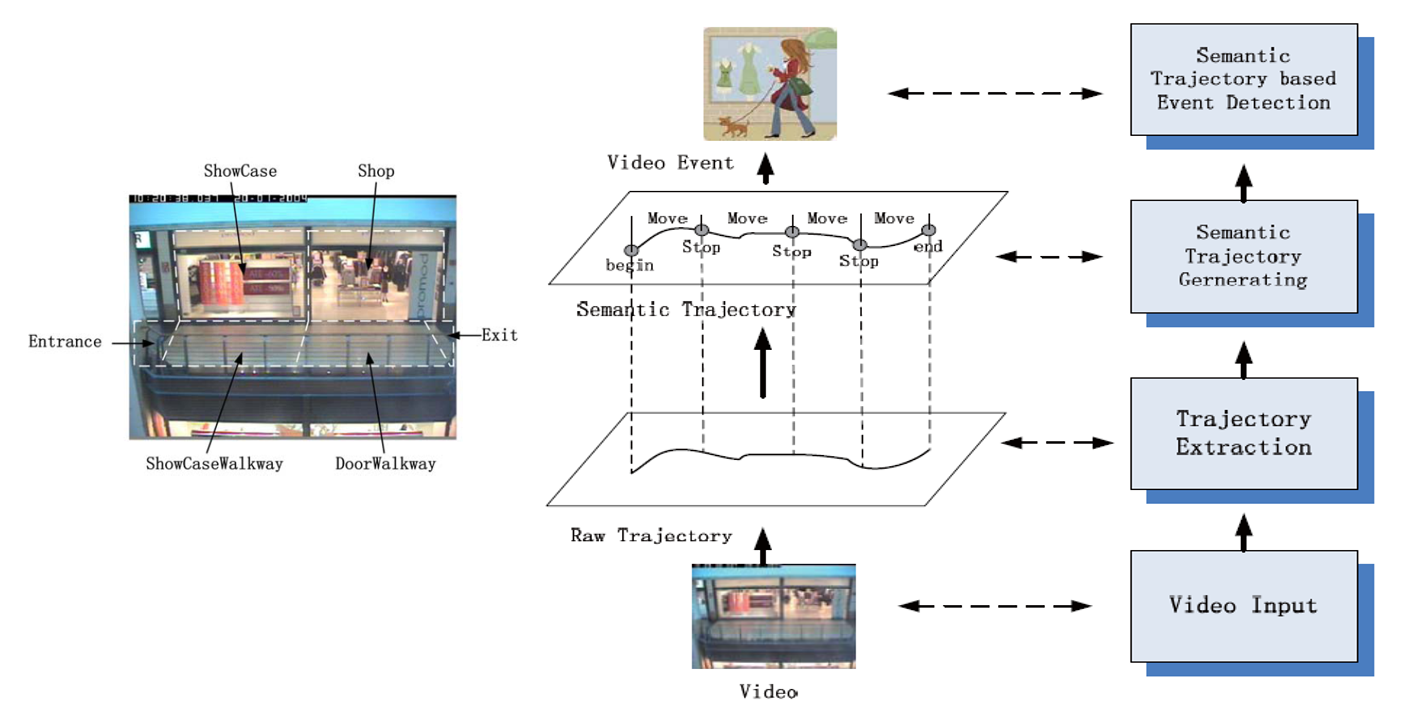
\includegraphics[width=1.0\textwidth]{figures//theme1//dsa_3.eps}
\end{figure}

\bibliographystyle{plain}
\nobibliography{tuliplab}
\footnotesize\bibentry{WLLS13J11}
\end{slide}
%%
%%==========================================================================================


%%==========================================================================================
%%

\begin{slide}[toc=,bm=]{Case Study (6) - Trajectory Analysis}
\begin{figure}[ht]
  \includemovie[poster=figures//theme1//Theme1_23.eps,inline=false]{12cm}{11cm}{figures//theme1//vs.avi}
\end{figure}
\end{slide}
%%
%%==========================================================================================


%%==========================================================================================
%%
\begin{slide}{Theme 2. Data Privacy}
%Theme two -
\begin{itemize}
\item
Information Abuse

\begin{itemize}
\item
The compromise of information
for which the data stakeholders are not willing to disclose

\item
It depends on the nature of the information,
the involved internal or external users,
and the ways in which the organization grants the access to
or releases the information

\end{itemize}
\end{itemize}

\end{slide}
%%
%%==========================================================================================


%%==========================================================================================
%%

\begin{slide}[toc=,bm=]{Theme 2. Data Privacy}

\twocolumn[
lcolwidth=0.5\linewidth,
rcolwidth=0.45\linewidth
]
{
\begin{itemize}
	\item
	Every user is potentially an adversary
	\begin{itemize}
		\item
		Once the data is released,
		we cannot prevent any user from performing any type of analysis on the released data
		\item
		Worst case scenario
		\begin{itemize}
			\item
			Must account for disclosure risk from any type of analyses
		\end{itemize}
	\end{itemize}
\end{itemize}
}
{	
	%\begin{figure}	
	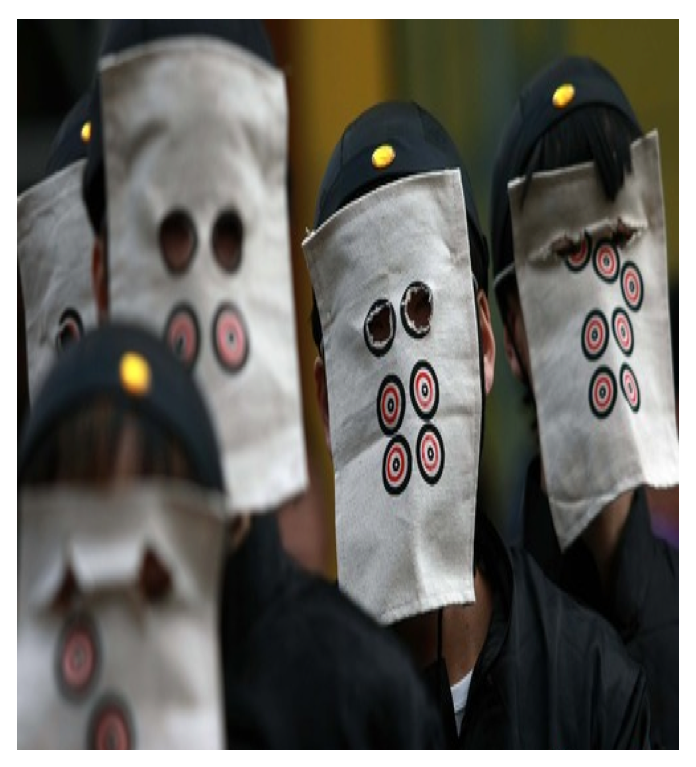
\includegraphics[width=\linewidth]{./figures/theme2/adversary.eps}
	%\end{figure}
}
	
\end{slide}
%%
%%==========================================================================================


%%==========================================================================================
%%
\begin{slide}[toc=,bm=]{Case Study (1) - Is O.S.N. a Secure Place to Show off?}
\begin{figure}[htbp]
	\centering
	\textbf{\large{\textcolor{orange}{Did Facebook photo trigger murder?}}}
	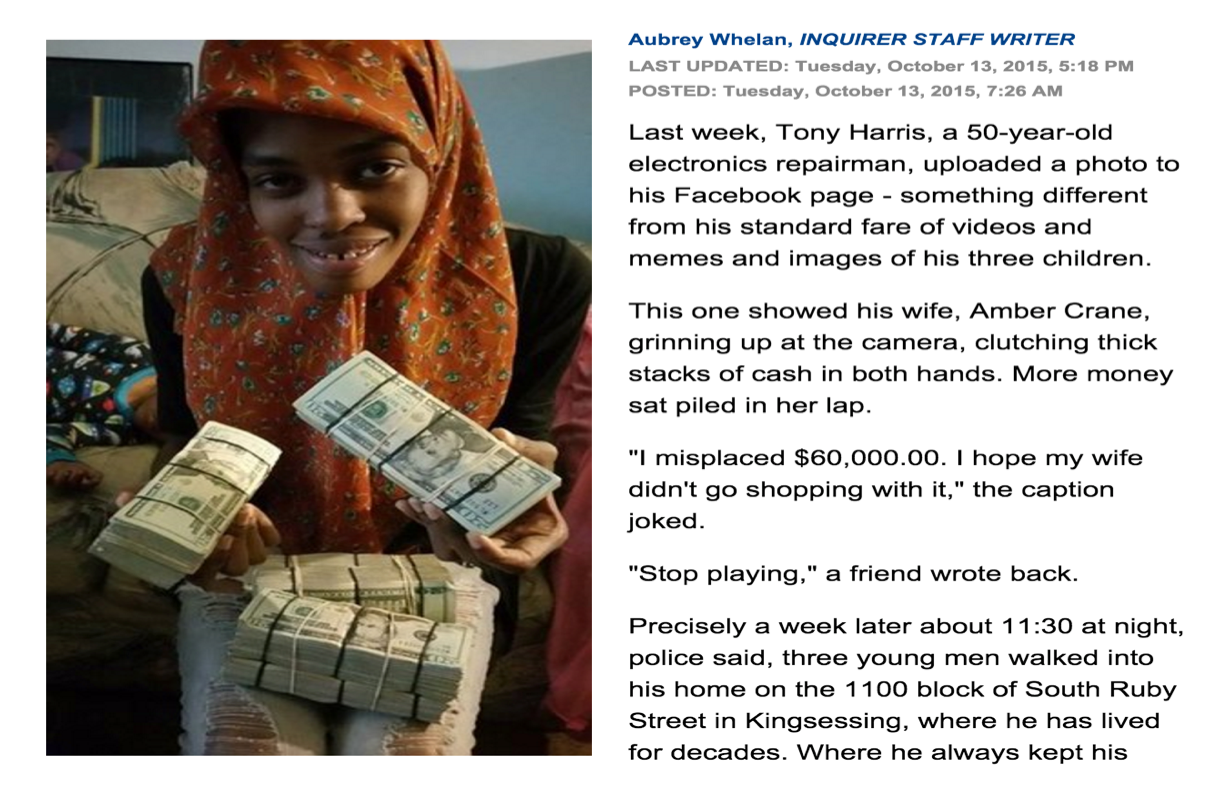
\includegraphics[width=0.7\textwidth,height=7cm]{./figures/theme2/case3.eps}
\end{figure}

\begin{thebibliography}{}
\bibitem{}
\small{Tianqing Zhu, Gang Li, Wanlei Zhou, Ping Xiong, and Cao Yuan.
Deferentially Private Tagging Recommendation Based on Topic Model. 
The 18th Pacific-Asia Conference on Knowledge Discovery and Data Mining (PAKDD),
May 2014, Tainan, Taiwan.}
\end{thebibliography}

\bibliographystyle{plain}
\nobibliography{tuliplab}
\footnotesize\bibentry{ZLZXY14C04}

\end{slide}
%%
%%==========================================================================================


%%==========================================================================================
%%
\iffalse
\begin{slide}[toc=,bm=]{Case Study (2) - Privacy Breach}
	%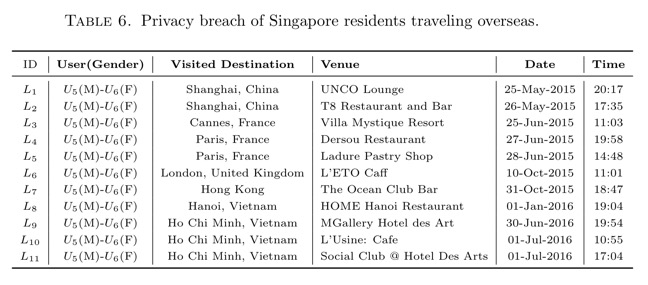
\includegraphics[width=\linewidth]{./figures/theme2/case1.jpg}
\begin{table}
	\fontsize{11pt}{11pt}\selectfont
	\setlength{\abovecaptionskip}{0pt}
	\setlength{\belowcaptionskip}{12pt}
	\centering
	\caption{Privacy breach of Singapore residents traveling overseas}
%	TABLE 6. Privacy breach of Singapore residents traveling overseas\protect\footnotemark[1].\\[15pt]
	\begin{tabular}{c|c|l|l|c|c}	
	\toprule
	ID  	&  	\textbf{User(Gender)}		& 		\textbf{Visited Destination} 		& 		\textbf{Venue} 		& 	\textbf{Date} 		&	\textbf{Time}	\\
	\midrule
	\rowcolor{orange}
	$L_1$	&	$U_5$(M)-$U_6$(F)	&	Shanghai, China 	   &	UNCO Lounge		&	25-May-2015	&	20:17\\
	\rowcolor{orange}
	$L_2$	&	$U_5$(M)-$U_6$(F)	&	Shanghai, China 	   &	T8 Restaurant and Bar		&	26-May-2015	&	17:35\\
	$L_3$	&	$U_5$(M)-$U_6$(F)	&	Cannes, France 	       &	Villa Mystique Resort		&	25-Jun-2015	&	11:03\\	
	\rowcolor{orange}
	$L_4$	&	$U_5$(M)-$U_6$(F)	&	Paris, France 		   &	Dersou Restaurant			&	27-Jun-2015	&	19:58\\
	\rowcolor{orange}
	$L_5$	&	$U_5$(M)-$U_6$(F)	&	Paris, France 		   &	Ladure Pastry Shop			&	28-Jun-2015	&	14:48\\
	$L_6$	&	$U_5$(M)-$U_6$(F)	&	London, United Kingdom &	L'ETO Caff			&	10-Oct-2015	&	11:01\\
	$L_7$	&	$U_5$(M)-$U_6$(F)	&	Hong Kong		       &	The Ocean Club Bar			&	31-Oct-2015	&	18:47\\
	$L_8$	&	$U_5$(M)-$U_6$(F)	&	Hanoi, Vietnam		   &	HOME Hanoi Restaurant			&	01-Jan-2016	&	19:04\\
	\rowcolor{orange}
	$L_9$	&	$U_5$(M)-$U_6$(F)	&	Ho Chi Minh, Vietnam   &	MGallery Hotel des Art		&	30-Jun-2016	&	19:54\\
	\rowcolor{orange}
	$L_{10}$&	$U_5$(M)-$U_6$(F)	&	Ho Chi Minh, Vietnam   &	L'Usine: Cafe		&	01-Jul-2016	&	10:55\\
	\rowcolor{orange}
	$L_{11}$&	$U_5$(M)-$U_6$(F)	&	Ho Chi Minh, Vietnam   &	Social Club @ Hotel Des Arts		&	01-Jul-2016	&	17:04\\
	\bottomrule
	\end{tabular}	
\end{table}

\bibliographystyle{plain}
\nobibliography{tuliplab}
\footnotesize\bibentry{VLLZ17J05}

\end{slide}
\fi

\begin{slide}[toc=,bm=]{Case Study (2) - Privacy Breach}

%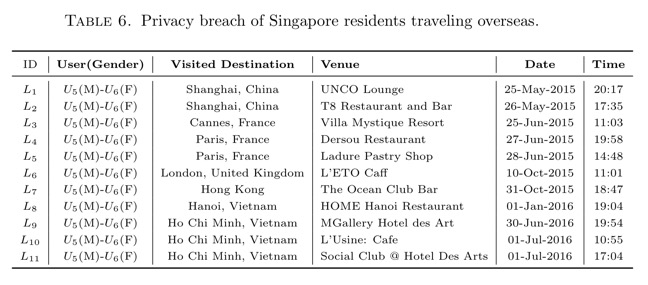
\includegraphics[width=\linewidth]{./figures/theme2/case1.jpg}
\begin{table}
	\fontsize{11pt}{11pt}\selectfont
	\setlength{\abovecaptionskip}{0pt}
	\setlength{\belowcaptionskip}{12pt}
	\centering
	\caption{Privacy breach of Singapore residents traveling overseas}
%	TABLE 6. Privacy breach of Singapore residents traveling overseas\protect\footnotemark[1].\\[15pt]
	\begin{tabular}{c|c|l|l|c|c}	
	\toprule
	ID  	&  	\textbf{User(Gender)}		& 		\textbf{Visited Destination} 		& 		\textbf{Venue} 		& 	\textbf{Date} 		&	\textbf{Time}	\\
	\midrule
	\onslide*{2,5}{\textcolor{orange}{$L_1$}}\onslide*{-1,3-4}{{$L_1$}}	
	&\onslide*{2,5}{\textcolor{orange}{$U_5$(M)-$U_6$(F)}}\onslide*{-1,3-4}{{$U_5$(M)-$U_6$(F)}}	
	&\onslide*{2,5}{\textcolor{orange}{Shanghai, China}}\onslide*{-1,3-4}{{Shanghai, China}} 	
	&\onslide*{2,5}{\textcolor{orange}{UNCO Lounge}}\onslide*{-1,3-4}{{UNCO Lounge}}				
	&\onslide*{2,5}{\textcolor{orange}{25-May-2015}}\onslide*{-1,3-4}{{25-May-2015}}
	&\onslide*{2,5}{\textcolor{orange}{20:17}}\onslide*{-1,3-4}{{20:17}}	\\
			
			
	\onslide*{2,5}{\textcolor{orange}{$L_2$}}\onslide*{-1,3-4}{{$L_2$}}	
	&\onslide*{2,5}{\textcolor{orange}{$U_5$(M)-$U_6$(F)}}\onslide*{-1,3-4}{{$U_5$(M)-$U_6$(F)}}	
	&\onslide*{2,5}{\textcolor{orange}{Shanghai, China}}\onslide*{-1,3-4}{{Shanghai, China}} 	
	&\onslide*{2,5}{\textcolor{orange}{T8 Restaurant and Bar}}\onslide*{-1,3-4}{{T8 Restaurant and Bar}}				
	&\onslide*{2,5}{\textcolor{orange}{26-May-2015}}\onslide*{-1,3-4}{{26-May-2015}}
	&\onslide*{2,5}{\textcolor{orange}{17:35}}\onslide*{-1,3-4}{{17:35}}	\\		
	
	$L_3$	&$U_5$(M)-$U_6$(F)	&Cannes, France 	       &Villa Mystique Resort		&25-Jun-2015	&11:03\\	
	
	\onslide*{3,5}{\textcolor{orange}{$L_4$}}\onslide*{-2,4}{{$L_4$}}	
	&\onslide*{3,5}{\textcolor{orange}{$U_5$(M)-$U_6$(F)}}\onslide*{-2,4}{{$U_5$(M)-$U_6$(F)}}	
	&\onslide*{3,5}{\textcolor{orange}{Paris, France }}\onslide*{-2,4}{{Paris, France}} 	
	&\onslide*{3,5}{\textcolor{orange}{Dersou Restaurant}}\onslide*{-2,4}{{Dersou Restaurant}}				
	&\onslide*{3,5}{\textcolor{orange}{27-Jun-2015}}\onslide*{-2,4}{{27-Jun-2015}}
	&\onslide*{3,5}{\textcolor{orange}{19:58}}\onslide*{-2,4}{{19:58}}	\\	
	
	\onslide*{3,5}{\textcolor{orange}{$L_5$}}\onslide*{-2,4}{{$L_5$}}	
	&\onslide*{3,5}{\textcolor{orange}{$U_5$(M)-$U_6$(F)}}\onslide*{-2,4}{{$U_5$(M)-$U_6$(F)}}	
	&\onslide*{3,5}{\textcolor{orange}{Paris, France }}\onslide*{-2,4}{{Paris, France}} 	
	&\onslide*{3,5}{\textcolor{orange}{Ladure Pastry Shop}}\onslide*{-2,4}{{Ladure Pastry Shop}}				
	&\onslide*{3,5}{\textcolor{orange}{28-Jun-2015}}\onslide*{-2,4}{{28-Jun-2015}}
	&\onslide*{3,5}{\textcolor{orange}{14:48}}\onslide*{-2,4}{{14:48}}	\\			
	
	
	$L_6$	&$U_5$(M)-$U_6$(F)	&London, United Kingdom 	&L'ETO Caff			&10-Oct-2015	&11:01\\
	$L_7$	&$U_5$(M)-$U_6$(F)	&Hong Kong		       		&The Ocean Club Bar			&31-Oct-2015	&18:47\\
	$L_8$	&$U_5$(M)-$U_6$(F)	&Hanoi, Vietnam		   	&HOME Hanoi Restaurant			&01-Jan-2016	&19:04\\
	
	\onslide*{4,5}{\textcolor{orange}{$L_9$}}\onslide*{-3}{{$L_9$}}	
	&\onslide*{4,5}{\textcolor{orange}{$U_5$(M)-$U_6$(F)}}\onslide*{-3}{{$U_5$(M)-$U_6$(F)}}	
	&\onslide*{4,5}{\textcolor{orange}{Ho Chi Minh, Vietnam}}\onslide*{-3}{{Ho Chi Minh, Vietnam}} 	
	&\onslide*{4,5}{\textcolor{orange}{MGallery Hotel des Art}}\onslide*{-3}{{MGallery Hotel des Art}}				
	&\onslide*{4,5}{\textcolor{orange}{30-Jun-2016}}\onslide*{-3}{{30-Jun-2016}}
	&\onslide*{4,5}{\textcolor{orange}{19:54}}\onslide*{-3}{{19:54}}	\\		
	
	
	\onslide*{4,5}{\textcolor{orange}{$L_{10}$}}\onslide*{-3}{{$L_{10}$}}	
	&\onslide*{4,5}{\textcolor{orange}{$U_5$(M)-$U_6$(F)}}\onslide*{-3}{{$U_5$(M)-$U_6$(F)}}	
	&\onslide*{4,5}{\textcolor{orange}{Ho Chi Minh, Vietnam}}\onslide*{-3}{{Ho Chi Minh, Vietnam}} 	
	&\onslide*{4,5}{\textcolor{orange}{L'Usine: Cafe}}\onslide*{-3}{{L'Usine: Cafe}}				
	&\onslide*{4,5}{\textcolor{orange}{01-Jul-2016}}\onslide*{-3}{{01-Jul-2016}}
	&\onslide*{4,5}{\textcolor{orange}{10:55}}\onslide*{-3}{{10:55}}	\\	
	
	\onslide*{4,5}{\textcolor{orange}{${L_{11}}$}}\onslide*{-3}{{$L_{11}$}}	
	&\onslide*{4,5}{\textcolor{orange}{$U_5$(M)-$U_6$(F)}}\onslide*{-3}{{$U_5$(M)-$U_6$(F)}}	
	&\onslide*{4,5}{\textcolor{orange}{Ho Chi Minh, Vietnam}}\onslide*{-3}{{Ho Chi Minh, Vietnam}} 	
	&\onslide*{4,5}{\textcolor{orange}{Social Club @ Hotel Des Arts}}\onslide*{-3}{{Social Club @ Hotel Des Arts}}				
	&\onslide*{4,5}{\textcolor{orange}{01-Jul-2016}}\onslide*{-3}{{01-Jul-2016}}
	&\onslide*{4,5}{\textcolor{orange}{17:04}}\onslide*{-3}{{17:04}}	\\		
	\bottomrule
	\end{tabular}
	
\end{table}

\begin{thebibliography}{}
\bibitem{}
\small{Huy Quan Vu, Gang Li, Rob Law, Yanchun Zhang.
Tourist Activity Analysis by Leveraging Mobile Social Media Data. 
Journal of Travel Research, 2017.}
\end{thebibliography}

\end{slide}
%%
%%==========================================================================================


%%==========================================================================================
%%
\begin{slide}[toc=,bm=]{Case Study (2) - Privacy Breach}
% - Case 2: Privacy Breach
%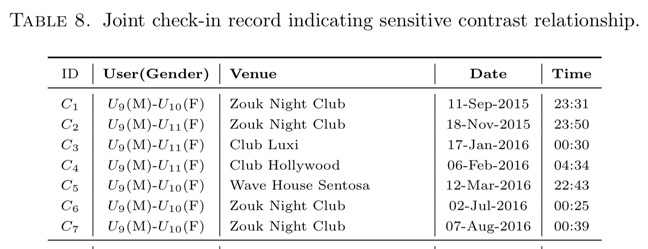
\includegraphics[width=\linewidth]{./figures/theme2/case2.jpg}

\begin{table}
	%\fontsize{11pt}{11pt}\selectfont
	\setlength{\abovecaptionskip}{0pt}
	\setlength{\belowcaptionskip}{12pt}
	\centering
	\caption{Joint check-in record indicating sensitive contrast relationship}
	%TABLE 8. Joint check-in record indicating sensitive contrast relationship\protect\footnotemark[1].\\[15pt]
	\begin{tabular}{c|c|l|c|c}	
\iffalse
	\toprule	
	ID  	&  	\textbf{User(Gender)}& 	\textbf{Venue} 		& 	\textbf{Date} 	&	\textbf{Time}	\\
	\midrule
	\rowcolor{orange}
	$C_1$	&	$U_9$(M)-$U_{10}$(F)	 &	Zouk Night Club		&	11-Sep-2015	    &	23:31\\
	\rowcolor{orange}
	$C_2$	&	$U_9$(M)-$U_{11}$(F)	 &	Zouk Night Club		&	18-Nov-2015	    &	23:50\\
	$C_3$	&	$U_9$(M)-$U_{11}$(F)	 &	Club Luxi			&	17-Jan-2016	    &	00:30\\
	$C_4$	&	$U_9$(M)-$U_{11}$(F)	 &	Club Hollywood		&	06-Feb-2016     &	04:34\\
	$C_5$	&	$U_9$(M)-$U_{10}$(F)	 &	Wave House Sentosa	&	12-Mar-2016	    &	22:43\\
	\rowcolor{orange}
	$C_6$	&	$U_9$(M)-$U_{10}$(F)	 &	Zouk Night Club		&	02-Jul-2016	    &	00:25\\
	\rowcolor{orange}
	$C_7$	&	$U_9$(M)-$U_{10}$(F)	 &	Zouk Night Club		&	07-Aug-2016	    &	00:39\\
	\bottomrule
\fi
	\toprule	
	ID  	&  	\textbf{User(Gender)}& 	\textbf{Venue} 		& 	\textbf{Date} 	&	\textbf{Time}	\\
	\midrule
	
	\onslide*{2,4}{\textcolor{orange}{$C_1$}}\onslide*{1,3}{{$C_1$}}	
	&\onslide*{2,4}{\textcolor{orange}{$U_9$(M)-$U_{10}$(F)}}\onslide*{1,3}{{$U_9$(M)-$U_{10}$(F)}}	
	&\onslide*{2,4}{\textcolor{orange}{Zouk Night Club}}\onslide*{1,3}{{Zouk Night Club}} 	
	&\onslide*{2,4}{\textcolor{orange}{11-Sep-2015}}\onslide*{1,3}{{11-Sep-2015}}				
	&\onslide*{2,4}{\textcolor{orange}{23:31}}\onslide*{1,3}{{23:31}}\\	
	
	\onslide*{2,4}{\textcolor{orange}{$C_2$}}\onslide*{1,3}{{$C_2$}}	
	&\onslide*{2,4}{\textcolor{orange}{$U_9$(M)-$U_{11}$(F)}}\onslide*{1,3}{{$U_9$(M)-$U_{11}$(F)}}	
	&\onslide*{2,4}{\textcolor{orange}{Zouk Night Club}}\onslide*{1,3}{{Zouk Night Club}} 	
	&\onslide*{2,4}{\textcolor{orange}{18-Nov-2015}}\onslide*{1,3}{{18-Nov-2015}}				
	&\onslide*{2,4}{\textcolor{orange}{23:50}}\onslide*{1,3}{{23:50}}\\	
		
	$C_3$	&$U_9$(M)-$U_{11}$(F)	 &Club Luxi			&17-Jan-2016	    &00:30\\
	$C_4$	&$U_9$(M)-$U_{11}$(F)	 &Club Hollywood		&06-Feb-2016     &04:34\\
	$C_5$	&$U_9$(M)-$U_{10}$(F)	 &Wave House Sentosa	&12-Mar-2016	    &22:43\\	
	
	\onslide*{3,4-}{\textcolor{orange}{$C_6$}}\onslide*{-2}{{$C_6$}}	
	&\onslide*{3,4-}{\textcolor{orange}{$U_9$(M)-$U_{10}$(F)}}\onslide*{-2}{{$U_9$(M)-$U_{10}$(F)}}	
	&\onslide*{3,4-}{\textcolor{orange}{Zouk Night Club}}\onslide*{-2}{{Zouk Night Club}} 	
	&\onslide*{3,4-}{\textcolor{orange}{02-Jul-2016}}\onslide*{-2}{{02-Jul-2016}}				
	&\onslide*{3,4-}{\textcolor{orange}{00:25}}\onslide*{-2}{{00:25}}\\	
	
	\onslide*{3,4}{\textcolor{orange}{$C_7$}}\onslide*{-2}{{$C_7$}}
	&\onslide*{3,4}{\textcolor{orange}{$U_9$(M)-$U_{10}$(F)}}\onslide*{-2}{{$U_9$(M)-$U_{10}$(F)}}
	&\onslide*{3,4}{\textcolor{orange}{Zouk Night Club}}\onslide*{-2}{{Zouk Night Club}} 	
	&\onslide*{3,4}{\textcolor{orange}{07-Aug-2016}}\onslide*{-2}{{07-Aug-2016}}				
	&\onslide*{3,4}{\textcolor{orange}{00:39}}\onslide*{-2}{{00:39}}\\	
	\bottomrule
		
	\end{tabular}
\end{table}

\begin{thebibliography}{}
\bibitem{}
\small{Huy Quan Vu, Gang Li, Rob Law, Yanchun Zhang.
Tourist Activity Analysis by Leveraging Mobile Social Media Data. 
Journal of Travel Research, 2017.}
\end{thebibliography}

\end{slide}
%%
%%==========================================================================================


%%==========================================================================================
%%
\begin{slide}[toc=,bm=]{Privacy Preserving Related Reference}

\twocolumn[
%lcolwidth=0.3\textwidth,
%rcolwidth=0.6\textwidth
lcolwidth=0.3\linewidth,
rcolwidth=0.65\linewidth
]
{
\begin{figure}[hbtp]
	%\raggedright
	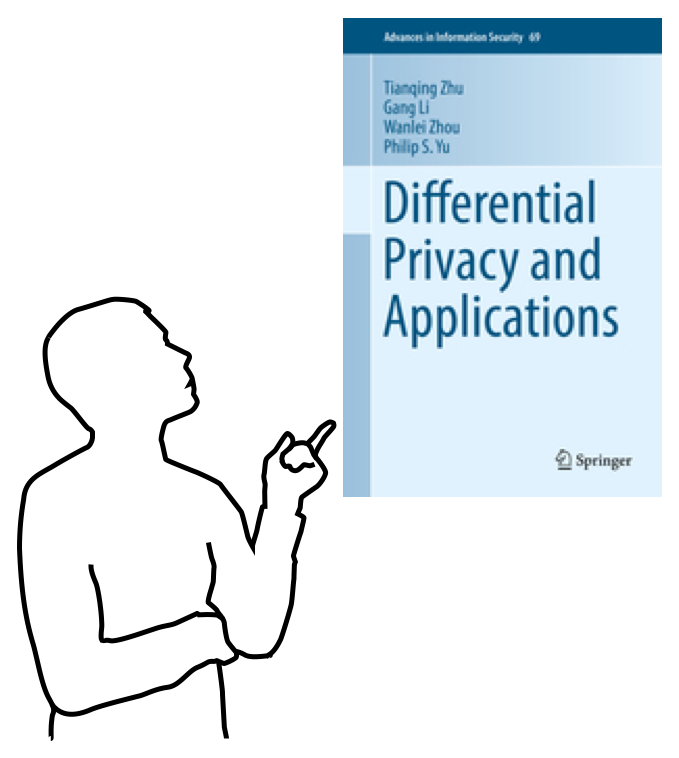
\includegraphics[scale=0.5]{./figures/theme2/reference.eps}
\end{figure}
}
{
\begin{itemize}
	\item
	\textbf{\underline{Privacy Preserving in Data Releasing}}
	\begin{itemize}
		\item
		T. Zhu, G. Li, W. Zhou, P.S. Yu. \textit{Differential Privacy and Its Applications: Survey}, \textbf{\uline{IEEE Transactions on Data and Knowledge Engineering}}, 2017
		\item
		T. Zhu, G. Li, W. Zhou, P.S. Yu. \textit{Differential Privacy and Its Applications}, Springer 2017
		\item
		T. Zhu, P. Xiong, G. Li, W. Zhou. \textit{Correlated Differential Privacy: Hiding Information in Non-IID Dataset}. \textbf{\uline{IEEE Transactions on Information Forensics \& Security}}, 2015, 10(2), 229-242
	\end{itemize}
\end{itemize}
}

\end{slide}
%%
%%==========================================================================================


%%==========================================================================================
%%

\begin{slide}{Theme 3. Business Intelligence}

\begin{itemize}
\item
Tourism Data Mining

\begin{itemize}
\item
Tourist Behavior Analysis

\item
Contrast Mining

\begin{itemize}

\item
Outlying Aspects Mining

\item
Competitiveness Discovery

\end{itemize}

\end{itemize}

\item
Recommendation System

\end{itemize}

\end{slide}
%%
%%==========================================================================================


%%==========================================================================================
%%
\begin{slide}[toc=,bm=]{Case Study (1) - Market Segmentation Analysis}
	%
	%%\begin{figure}[htbp]
	%%	\subfigure{
	%%		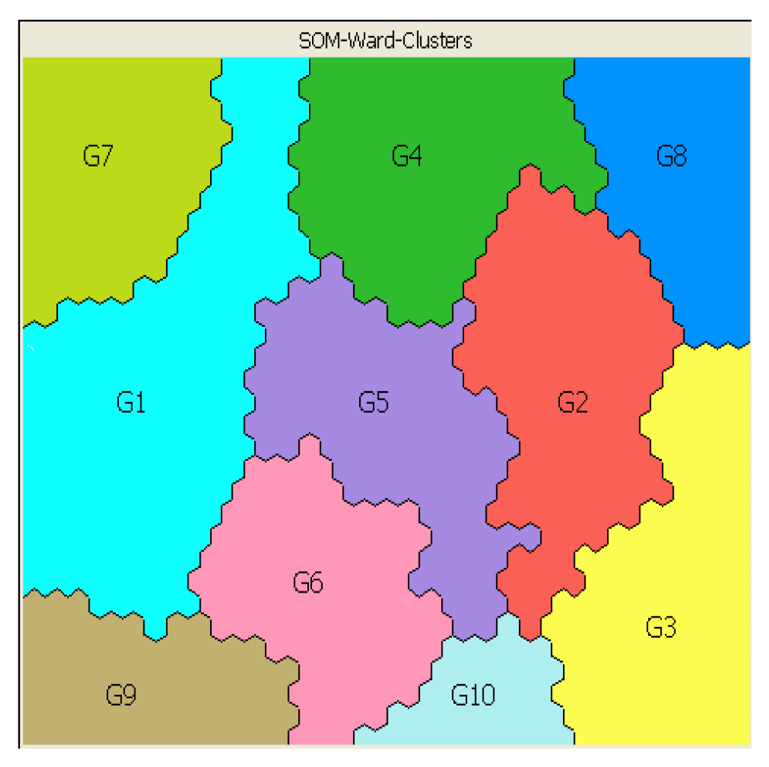
\includegraphics[width=0.4\textwidth]{figures//theme3//Theme3_1.eps}
	%%	}
	%%	\subfigure{
	%%		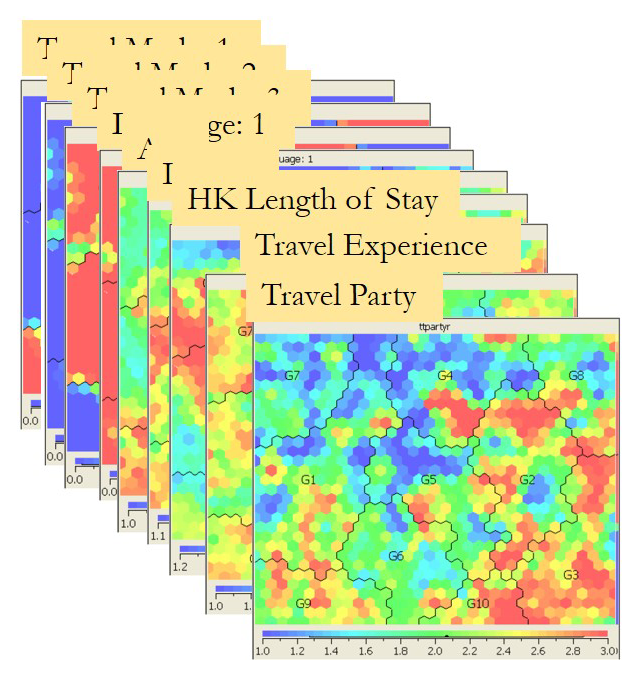
\includegraphics[width=0.4\textwidth]{figures//theme3//Theme3_2.eps}
	%%	}
	%%\end{figure}
	%
	%\twocolumn{
	%	\begin{figure}
	%%		\begin{overprint}
	%		\onslide*{1, 1-}{
	%			\put(-100,50){
	%				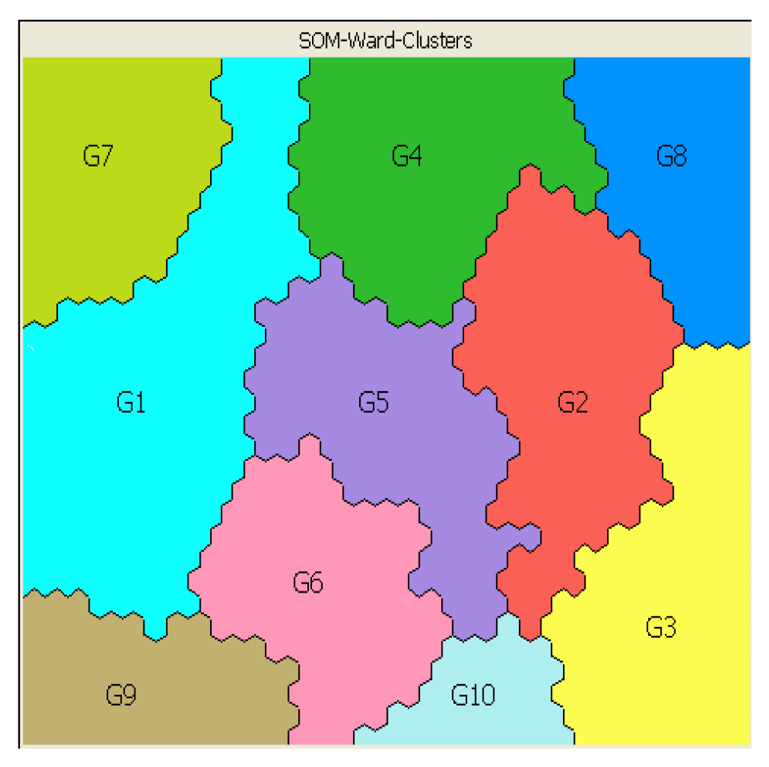
\includegraphics[width=0.9\textwidth]{figures//theme3//Theme3_1_1_1.eps}
	%			}
	%		}
	%		\onslide*{3, 3-}{
	%			\put(-100,50){
	%				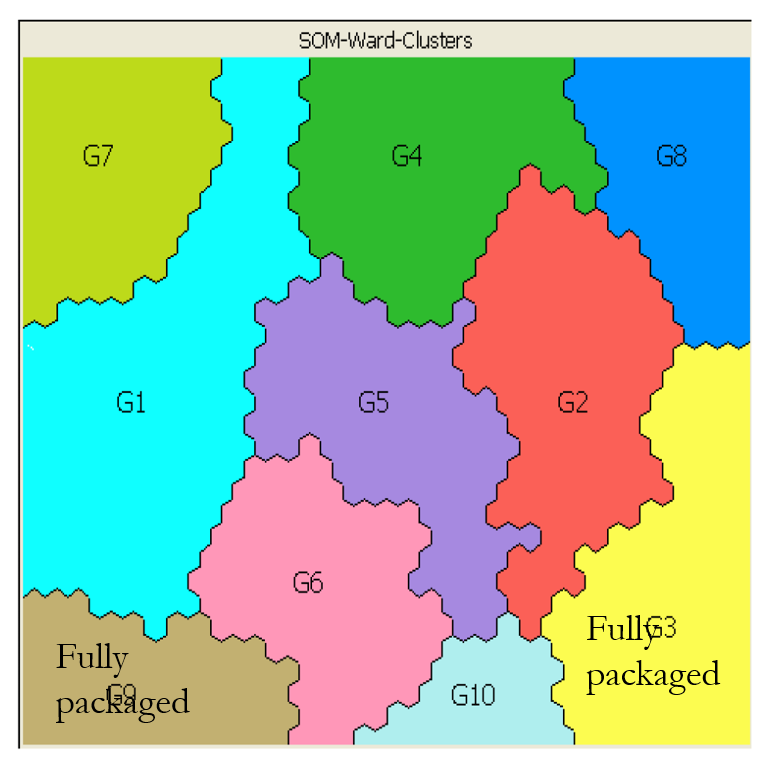
\includegraphics[width=0.9\textwidth]{figures//theme3//Theme3_1_1_2.eps}
	%			}
	%%			\parbox[10,9]{5em}{Fully packaged}
	%%			\parbox[-80,9]{5em}{Fully packaged}
	%		}
	%		\onslide*{5, 5-}{
	%			\put(-100,50){
	%				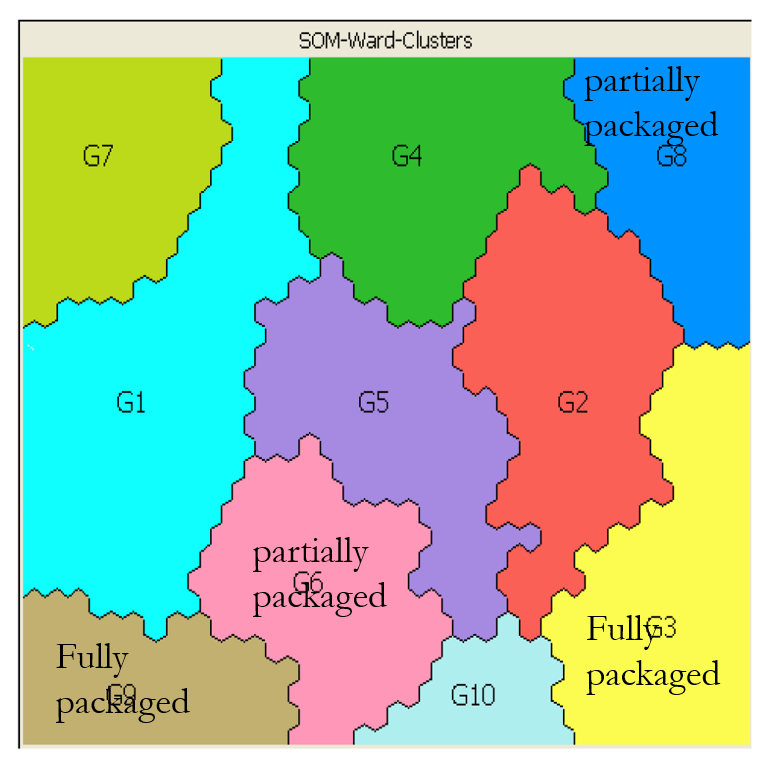
\includegraphics[width=0.9\textwidth]{figures//theme3//Theme3_1_1_3.eps}
	%			}		
	%%			\parbox[30,0]{5em}{Partially packaged}
	%%			\parbox[18,6]{5em}{Partially packaged}
	%		}
	%		\onslide*{9, 9-}{
	%			\put(-100,50){
	%				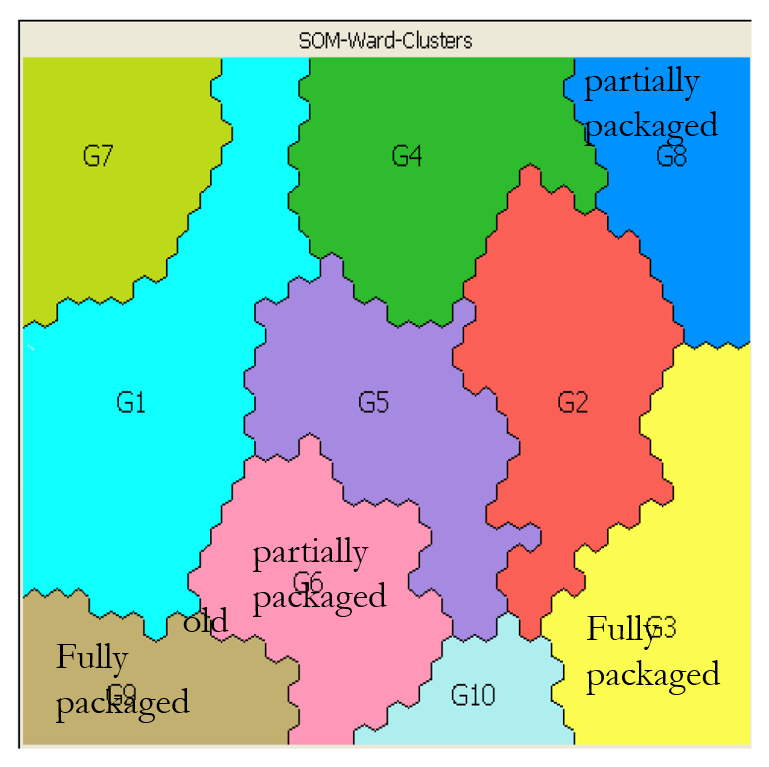
\includegraphics[width=0.9\textwidth]{figures//theme3//Theme3_1_1_4.eps}
	%			}
	%%			\parbox[0,10]{5em}{old}
	%%
	%		}
	%		\onslide*{11, 11-}{
	%			\put(-100,50){
	%				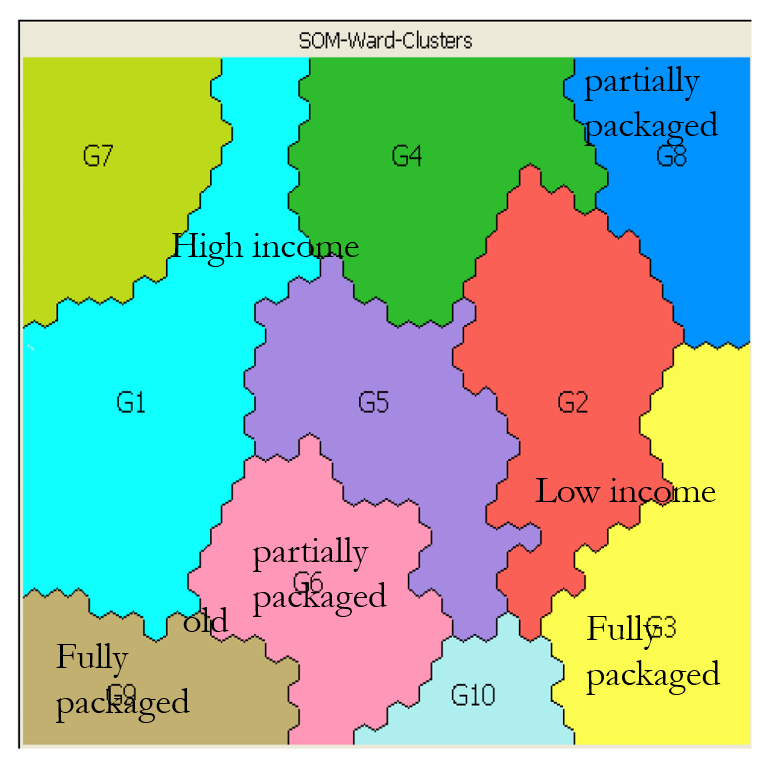
\includegraphics[width=0.9\textwidth]{figures//theme3//Theme3_1_1_5.eps}
	%			}
	%%			\parbox[10,10]{5em}{High income}
	%%			\parbox[20,10]{5em}{High income}
	%		}
	%%		\end{overprint}
	%	\end{figure}
	%}
	%{
	%\centering
	%	\begin{figure}
	%%		\begin{overprint}
	%		\onslide*{2, 2-}{
	%			\put(-110,90){
	%				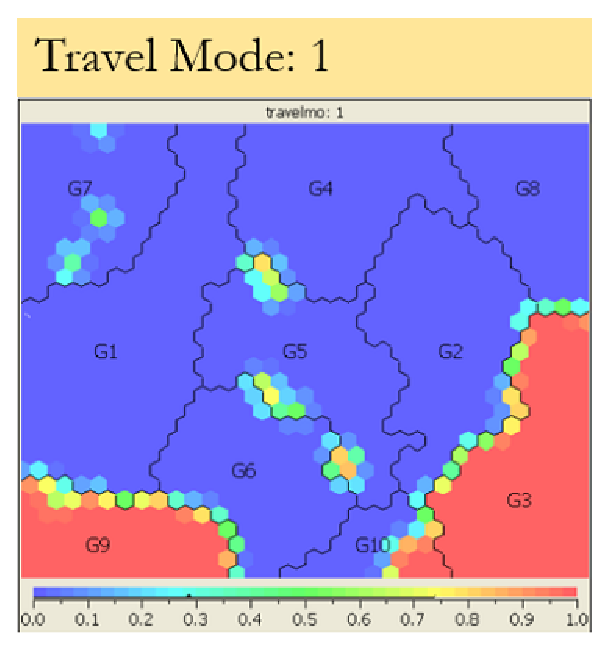
\includegraphics[width=0.7\textwidth]{figures//theme3//Theme3_1_2.eps}
	%			}
	%		}
	%		\onslide*{4, 4-}{
	%			\put(-100,80){
	%				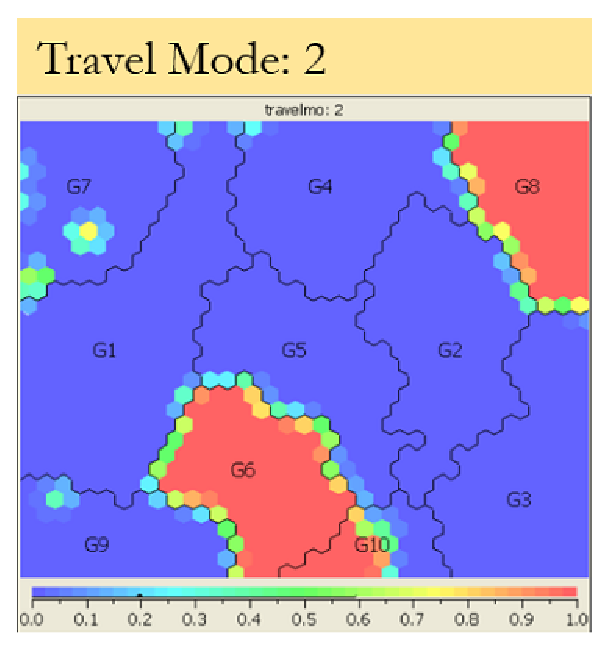
\includegraphics[width=0.7\textwidth]{figures//theme3//Theme3_1_3.eps}
	%			}
	%		}
	%		\onslide*{6, 6-}{
	%			\put(-90,70){
	%				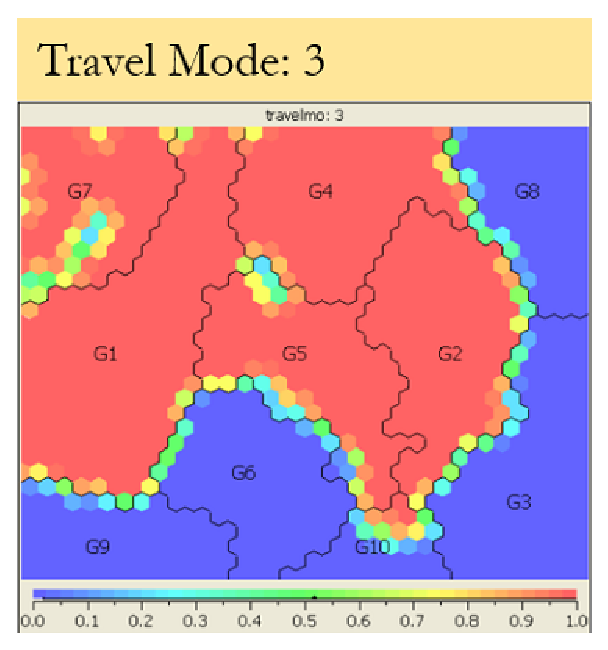
\includegraphics[width=0.7\textwidth]{figures//theme3//Theme3_1_4.eps}
	%			}
	%		}
	%		\onslide*{7, 7-}{
	%			\put(-80,60){
	%				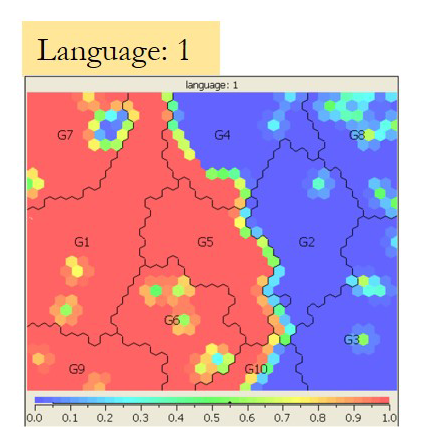
\includegraphics[width=0.7\textwidth]{figures//theme3//Theme3_1_5.eps}
	%			}
	%		}
	%		\onslide*{8, 8-}{
	%			\put(-70,50){
	%				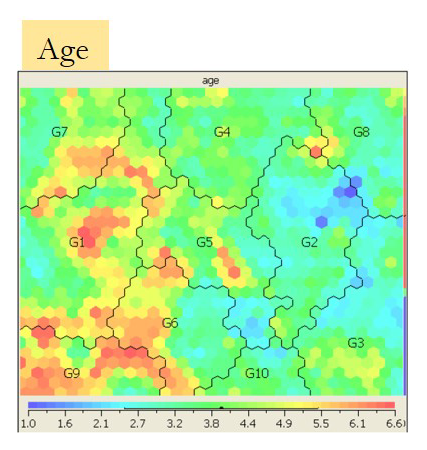
\includegraphics[width=0.7\textwidth]{figures//theme3//Theme3_1_6.eps}
	%			}
	%		}
	%		\onslide*{10, 10-}{
	%			\put(-60,40){
	%				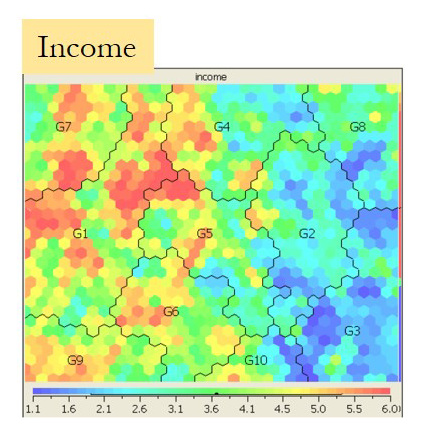
\includegraphics[width=0.7\textwidth]{figures//theme3//Theme3_1_7.eps}
	%			}
	%		}
	%		\onslide*{12, 12-}{
	%			\put(-50,30){
	%				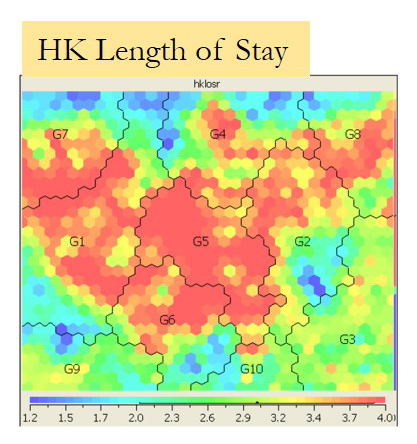
\includegraphics[width=0.7\textwidth]{figures//theme3//Theme3_1_8.eps}
	%			}
	%		}
	%		\onslide*{13, 13-}{
	%			\put(-40,20){
	%				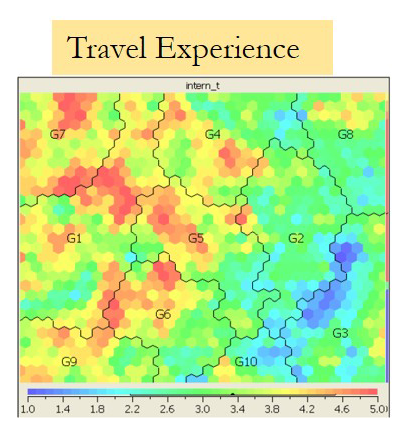
\includegraphics[width=0.7\textwidth]{figures//theme3//Theme3_1_9.eps}
	%			}
	%		}
	%		\onslide*{14, 14-}{
	%			\put(-30,10){
	%			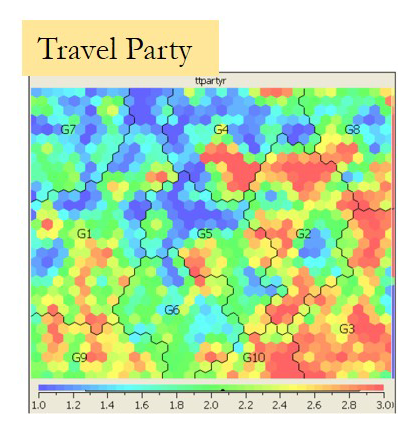
\includegraphics[width=0.7\textwidth]{figures//theme3//Theme3_1_10.eps}
	%				}	
	%		}
	%%		\end{overprint}
	%	\end{figure}
	%}
	%\vspace*{-20pt}
	%
	%\bibliographystyle{plain}
	%\nobibliography{tuliplab}
	%\footnotesize\bibentry{LLW10J03}
	%
\end{slide}
%%
%%==========================================================================================


%%==========================================================================================
%%
\begin{slide}[toc=,bm=]{Case Study (2) - Negative Association Rule Mining}
	\selectcolormodel{rgb}
	\usetikzlibrary{positioning}
	\tikzstyle{block} = [rectangle, draw=orange, fill= orange!20, text width=7em, text centered, rounded corners, minimum height=4em,font=\small]
	\tikzstyle{line} = [draw, -latex']
	\tikzstyle{note} = [rectangle, text width=10em, text centered, rounded corners, minimum height=0.5em,font=\footnotesize]
	\vspace*{-20pt}
	\begin{center}
		\begin{tikzpicture}[node distance = 1cm and 1.5cm, auto]
		\node[block](initialTransData){Transcation Data};
		\node[block,right= of initialTransData](candiPosItem){Candidate Interesting \textbf{Positive} Item-set};
		\node[block, below= of initialTransData](initialUserItem){User specified Target Item};
		\node[block,right= of initialUserItem](generateItem){Generating Targeted Item-set};
		
		\node[block, below= of generateItem](candiNegItem){Candidate Interesting \textbf{Negative} Item-set};
		\node[block, right= of candiNegItem](interNegItem){Interesting Negative Item-set};
		\node[block, right= of interNegItem](negRule){Negative Rules};
		
		\node[block, right= of candiPosItem](interPosItem){Interesting Positive Item-set};
		\node[block, right= of interPosItem](posRule){Positive Rules};
		\node[block, below= of posRule](report){Reporting Rules};
		
		\path[line](initialTransData) -- (generateItem);
		\path[line](initialUserItem) -- (generateItem);
		\path[line](generateItem) -- (candiPosItem);
		\path[line](candiPosItem) -- (interPosItem);
		\path[line](interPosItem) -- (posRule);
		\path[line](posRule) -- (report);
		\path[line](generateItem) -- (candiNegItem);
		\path[line](candiNegItem) -- (interNegItem);
		\path[line](interNegItem) -- (negRule);
		\path[line](negRule) -- (report);
		
		\begin{scope}[node distance = 0.5cm, auto]
		\node[note, above= of candiPosItem](candiPosItemNote){$Sup(A\cup B)\geq min\_ sup$};
		\node[note, above= of interPosItem](interPosItemNote){$lever(A\cup B)\geq <min\_ lever$};
		\node[note, above= of posRule](posRuleNote){$confi(A\to \sim B)\geq <min\_ confi$};
		\node[note, below= of candiNegItem](candiNegItemNote){$Sup(A\cup B)<min\_ sup$};
		\node[note, below= of interNegItem](interNegItemNote){$lever(A\cup \sim B)\geq <min\_ lever$};
		\node[note, below= of negRule](negRuleNote){$confi(A\to \sim B)\geq <min\_ confi$};	
		\end{scope}
		
		
		\end{tikzpicture}
	\end{center}
	%\vspace*{-15pt}
	
	\bibliographystyle{plain}
	\nobibliography{tuliplab}
	\footnotesize\bibentry{RVLL11J06}
	
\end{slide}
%%
%%==========================================================================================


%%==========================================================================================
%%
\begin{slide}[toc=,bm=]{Case Study (3) - Contrast Mining}
	%	
	%	\twocolumn[lcolwidth=0.55\linewidth,
	%	rcolwidth=0.45\linewidth
	%	]{
	%
	%\begin{itemize}
	%	\item Contrast Targeted Rules Algorithm (CTR):
	%	\vspace{0.5cm}		
	%		\begin{itemize}
	%			\item
	%			Detect the changes of rules strength
	%			between differences year data set.
	%			
	%			\item
	%			Tracing  the trend for predicting
	%			future potential.
	%			
	%		\end{itemize}
	%	\end{itemize}
	%	}
	%	{
	%		\begin{center}
	%			\begin{figure}[htbp]
	%				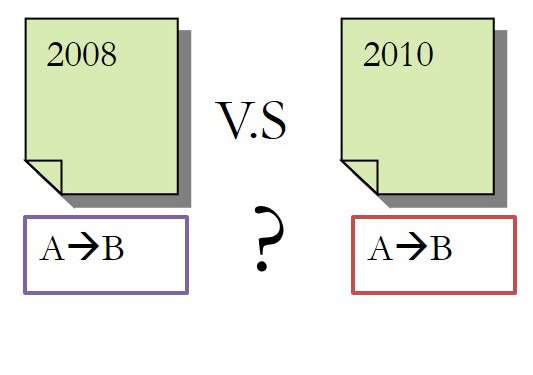
\includegraphics[height=0.75\textheight]{figures//theme3//Theme3_3_1.eps}
	%			\end{figure}
	%		\end{center}
	%		
	%	}
	%\vspace*{-40pt}
	%	\twocolumn[lcolwidth=0.6\linewidth,rcolwidth=0.4\linewidth,colsep=0.001\linewidth]{
	%	\begin{figure}[htbp]
	%		\onslide*{2, 2-}
	%		{
	%			\subfigure{
	%				\includegraphics[height=0.65\textheight]{figures//theme3//Theme3_3_2.eps}
	%			}
	%		}
	%
	%	\end{figure}
	%	}
	%	{
	%		\begin{figure}
	%			
	%			\onslide*{3, 3-}{
	%				\subfigure{
	%					\includegraphics[height=0.65\textheight]{figures//theme3//Theme3_3_3.eps}
	%				}
	%			}	
	%		\end{figure}
	%
	%	}
	%\vspace*{\fill}
	%
	%\bibliographystyle{plain}
	%\nobibliography{tuliplab}
	%\footnotesize\bibentry{RVLL11J06}
	%
\end{slide}
%%
%%==========================================================================================


%%==========================================================================================
%%
\begin{slide}[toc=,bm=]{Case Study (4) - PR Based Conditional Random Fields}
	
	\begin{itemize}
		\item  \textbf{Heterogeneous Preferences}
		
		\begin{itemize}
			\item \textbf{User-wise biases}
			%	\setlength\itemsep{-0.5em}
			\begin{itemize}
				%	\setlength\itemsep{-0.3em}
				\item Users give lower ratings when in bad mood
				
				\item Different scales, e.g., 4/5 $($ Shown in Table 3$)$ star is ``OK'' for critics
				
				\item User interface design
				
			\end{itemize}
			
			\item \textbf{Item-wise biases}
			
			%	\setlength\itemsep{-0.5em}
			\begin{itemize}
				
				\item The same item presented differently,
				e.g., a movie in 3D, HD
				
			\end{itemize}
		\end{itemize}
	\end{itemize}
	
	\vspace*{-45pt}
	\begin{table}[h]
		\fontsize{11pt}{11pt}\selectfont
		\setlength{\abovecaptionskip}{0pt}
		\setlength{\belowcaptionskip}{1pt}
		\centering
		\caption{the user-item rating matrix.}
		\begin{threeparttable}
			\begin{tabular}{l|c|c|c|c}	
			\toprule
			\textbf{User$\backslash$Movie}  	&  	\textbf{Spider\-Man}		& 		\textbf{2012} 		& 		\textbf{The Godfather} 		& 	\textbf{The Social Network}\\
			\midrule
			Bob	&	3	&	2 	&	4	&	5	\\
			Justin	&	?	&	5   &	2	&	?	\\
			John	&	4	&	4 	&	2	&	1	\\
			Larry	&	3	&	3 	&	4	&	2	\\
			Cindy	&	4	&	3 	&	4	&	1	\\
			Paul	&	2	&	3 	&	4	&	?	\\
			David	&	3 \tnote{1}	&	? \tnote{2}	&	4	&	1	\\
			\bottomrule
		\end{tabular}
		\begin{tablenotes}
			\item[1] Rating
			\item[2] No rating Question: will David like 2012?
		\end{tablenotes}
	\end{threeparttable}

\end{table}

\begin{tablenotes}
	\item[1] Rating
	\item[2] No rating Question: will David like 2012?
\end{tablenotes}
\end{slide}
%%
%%==========================================================================================


%%==========================================================================================
%%
\begin{slide}[toc=,bm=]{Case Study (4) - PR Based Conditional Random Fields}

\begin{figure}
	\includegraphics[width=0.8\textwidth]{figures//theme3//Theme3_5_1.eps}
\end{figure}

\bibliographystyle{plain}
\nobibliography{tuliplab}
\footnotesize\bibentry{LLTJ16J02}

\end{slide}

%%
%%==========================================================================================


%%==========================================================================================
%%
\begin{slide}{Research Publications}
\onslide*{-1}
{\vspace{1.5cm}
\begin{table}
\fontsize{11pt}{11pt}\selectfont
    \begin{tabular}{c|c c c|c c c}
    \toprule
\cmidrule{1-1}    \multirow{2}[4]{*}{Year} & \multicolumn{3}{c|}{SCI/SSCI Journals} &
\multicolumn{3}{c}{Referred Conferences} \\
\cmidrule{2-7}          & Q1 (71\%) & Q2 (18\%) & Q3 (11\%) & A (16\%) & B (9\%) & C (75\%) \\
    \midrule
    2018  & 9     & 1     & 2     & 0     & 1     & 4 \\
    2017  & 6     & 2     & 1     & 0     & 0     & 6 \\
    2016  & 2     & 3     & 1     & 0     & 0     & 5 \\
    2015  & 6     & 4     & 1     & 0     & 1     & 2 \\
    2014  & 10    & 0     & 2     & 0     & 0     & 4 \\
    2013  & 11    & 1     & 0     & 3     & 2     & 2 \\
    2012  & 2     & 1     & 2     & 4     & 1     & 2 \\
    2011  & 7     & 1     & 1     & 0     & 0     & 2 \\
    2010  & 4     & 1     & 0     & 2     & 0     & 1 \\
    2009  & 1     & 1     & 0     & 0     & 0     & 4 \\
    2008  & 3     & 0     & 0     & 0     & 0     & 6 \\
    2007  & 1     & 0     & 0     & 0     & 0     & 3 \\
    2006  & 0     & 0     & 0     & 0     & 0     & 2 \\
    \bottomrule
    \end{tabular}
\end{table}
}

\onslide*{2}
{\vspace{1.5cm}
\begin{center}
\selectcolormodel{rgb}
\begin{tikzpicture}
    \begin{axis}[
        title={SCI/SSCI Journals},
        %xlabel={right: $years$},
        ylabel=number of papers,
        ytick={0,2,4,6,8,10,12,14},
        x tick label style={rotate=75,anchor=east},
        legend pos=north west]
    \addplot[mark=*,blue!50] plot coordinates {
    (2006,0)(2007,1)(2008,3)(2009,2)(2010,5)(2011,9)
    (2012,5)(2013,12)(2014,12)(2015,11)(2016,6)(2017,9)(2018,12)
    };

    \addlegendentry{\tiny{SCI/SSCI Journals}}

    \addplot[color=orange,mark=square]
    plot coordinates {
    (2006,2)(2007,3)(2008,6)(2009,4)(2010,3)(2011,2)(2012,7)
    (2013,7)(2014,4)(2015,3)(2016,5)(2017,6)(2018,5)
    };
    \addlegendentry{\tiny{Referred Conferences}}
    \end{axis}
    \end{tikzpicture}
\end{center}
}

\end{slide}
%%
%%==========================================================================================


%%==========================================================================================
%%
\begin{slide}{Research Awards}
\vspace{2.2cm}
\begin{table}[htbp]
  \centering
    \begin{tabular}{ r | l | r  r }
    \toprule
    \multicolumn{1}{ l |}{\textbf{Year}} & \textbf{Awards} & \textbf{Author} &  \\
    \midrule
    \textbf{2018} & KSEM 2018 Best Paper Award & Shaoni Wang &  \\

    \textbf{2017} & IFITT Journal Paper of The Year Award (1st Prize) & Huy Quan Vu &  \\

    \textbf{2016} & IEEE TrustCom 2016 Best Student Paper Award & Na Pang &  \\

    \textbf{2015} & IFITT Journal Paper of The Year Award (3rd Prize) & Huy Quan Vu &  \\

    \textbf{2014} & PAKDD 2014 Best Student Paper Award & Tianqing Zhu &  \\

    \textbf{2012} & ACM ASONAM 2012  Best Paper Award & Yongli Ren &  \\

    \textbf{2007} & MBEC 2007 Springer Nightingale Prize & Jingyu Hou &  \\
    \bottomrule
    \end{tabular}
  \label{tab:addlabel}
\end{table}

\end{slide}
%%
%%==========================================================================================


%%==========================================================================================
%%
%\begin{slide}[toc=,bm=]{Research Awards}
%
%\begin{figure}
%%		\begin{overprint}
%		\onslide*{2, 2-}{
%			\put(-280,90){
%				\includegraphics[width=0.3\textwidth]{figures//awards//TULIPAwards2018B.eps}
%			}
%		}
%		\onslide*{2, 2-}{
%			\put(-100,90){
%				\includegraphics[width=0.3\textwidth]{figures//awards//TULIPAwards2018A.eps}
%			}
%		}
%		\onslide*{2, 2-}{
%			\put(80,90){
%				\includegraphics[width=0.35\textwidth]{figures//awards//TULIPAwards2016A.eps}
%			}
%		}
%		\onslide*{3, 3-}{
%			\put(-160,-40){
%				\includegraphics[width=0.25\textwidth]{figures//awards//TULIPAwards2012.eps}
%			}
%		}
%		\onslide*{3, 3-}{
%			\put(30,-40){
%				\includegraphics[width=0.25\textwidth]{figures//awards//TULIPAwards2007.eps}
%			}
%		}
%		\onslide*{4, 4-}{
%			\put(-250,-80){
%				\includegraphics[width=0.35\textwidth]{figures//awards//TULIPAwards2016B.eps}
%			}
%		}
%		\onslide*{4, 4-}{
%			\put(80,-80){
%				\includegraphics[width=0.35\textwidth]{figures//awards//TULIPAwards2014.eps}
%			}
%		}
%	\end{figure}
%
%\end{slide}
%%
%%==========================================================================================


\section{Training @ TULIP}


%%%==========================================================================================
%%%
%\begin{slide}{Roadmap}
%\begin{itemize}
%  \item \textcolor{orange}{Professional knowledge}
%    \begin{itemize}
%          \item \LaTeX{},
%                Version Control System (\texttt{SmartGit Github Bitbucket})
%          \item Plan \& Progress Review
%          \item References Management
%        \end{itemize}
%  \item \textcolor{orange}{Foundational Knowledge}
%    \begin{itemize}
%      \item FLIP (00)\texttildelow FLIP (05)
%    \end{itemize}
%  \item \textcolor{orange}{Research Skills}
%    \begin{itemize}
%      \item Review Team
%      \item Reading Team
%        \begin{itemize}
%          \item QQ Online
%          \item At least once a month
%          \item Read material before meeting,
%                ask questions.
%        \end{itemize}
%    \end{itemize}
%\end{itemize}
%%\gangli{this seems close to that mind map}
%\end{slide}
%%%
%%%==========================================================================================


%%%==========================================================================================
%%%
%\begin{slide}[toc=,bm=]{Training at TULIP}
%    \begin{itemize}
%      \item Learning content (FLIP (00)\texttildelow FLIP (05))
%        \begin{enumerate}
%          \item \textcolor{orange}{Mathematics}
%            \begin{itemize}
%              \item Linear algebra,
%                    Probability theory,
%                    Mathematical statistics
%            \end{itemize}
%          \item \textcolor{orange}{Hand-on Skills}
%            \begin{itemize}
%              \item Python,
%                    Apache Spark,
%                    Cloud platform
%            \end{itemize}
%          \item \textcolor{orange}{Learning theoretical knowledge}
%            \begin{itemize}
%              \item Optimization,
%                    Graph model
%            \end{itemize}
%          \item \textcolor{orange}{Professional Knowledge}
%        \end{enumerate}
%    \end{itemize}
%\end{slide}
%%%
%%%==========================================================================================


%%==========================================================================================
%%
\begin{slide}{Roadmap}
\begin{center}

\selectcolormodel{rgb}
   \begin{tikzpicture}[ every annotation/.style = {draw,
                     fill = white}]
  \path[mindmap,concept color=blue!40,text=white,
    every node/.style={concept},
    root/.style    = {concept color=black!40,
      font=\Large\bfseries,text width=10em},
    level 1 concept/.append style={font=\bfseries,
      sibling angle=100,text width=7.7em,level distance=8em,inner sep=0pt},
    level 2 concept/.append style={font=\sf,text width=5em,inner sep=0pt},
  ]
  node[root,scale=0.6, concept color=blue!50,text=white] {Training at TULIP} [clockwise from=180]
    child[concept color=orange!60] {
      node[scale=0.6] {Professional knowledge} [clockwise from=260]
        child { node[scale=0.6] {\LaTeX} }
        child { node[scale=0.6] (goReview) {Plan \& Progress Review }}
        child { node[scale=0.6] (goRefrences ){References Management}}
        child { node[scale=0.6] (goVersionCon) {Version Control System}}
    }
     child[concept color=blue!60] {
      node[concept,scale=0.6] {Foundation (FLIP(00-05))}[clockwise from=160]
      child{node[concept,scale=0.6](hand-on){Hand-on Skills}}
      child{node[concept,scale=0.6](Professional){Professional Knowledge}}
      child{node[concept,scale=0.6](Theo){Theoretical knowledge}}
      child{node[concept,scale=0.6](Math){Mathmatics}}
    }
    child[concept color=blue!60] {
      node[concept,scale=0.6] {Research Skills}
        [clockwise from=60]
      child { node[concept,scale=0.6] (TeXampleBlog)
        {Reading Team} }
      child { node[concept,scale=0.6] (Reviewteam)
        {Review Team }}
    }
   ;
    \info{goVersionCon.north west}{above,anchor=east,xshift=-0.5em}{%
      \item SmartGit
      \item GitHub
      \item Bitbucket
    }
    \end{tikzpicture}
\end{center}
%%==========================================================================================
\begin{note}
Professional knowledge: \LaTeX, Version Control Systems
(SmartGit  GitHub Bitbucket), Plan \& Progress Review, References Management\\
Foundational Knowledge: FLIP(00): Data Science,
FLIP(01): Advanced Data Science,
FLIP(02): Modern Data Science,
FLIP(03): Deep Learning,
FLIP(04): Learning Theory (I),
FLIP(05): Learning Theory (II)\\
Research Skills: Review Team, Reading Team
\end{note}
%%==========================================================================================
\end{slide}
%%
%%==========================================================================================

%%==========================================================================================
%%
\begin{slide}[toc=,bm=]{Roadmap}
\begin{center}

\selectcolormodel{rgb}
   \begin{tikzpicture}[ every annotation/.style = {draw,
                     fill = white}]
  \path[mindmap,concept color=blue!40,text=white,
    every node/.style={concept},
    root/.style    = {concept color=black!40,
      font=\Large\bfseries,text width=10em},
    level 1 concept/.append style={font=\bfseries,
      sibling angle=100,text width=7.7em,level distance=8em,inner sep=0pt},
    level 2 concept/.append style={font=\sf,text width=5em,inner sep=0pt},
  ]
  node[root,scale=0.6, concept color=blue!50,text=white] {Training at TULIP} [clockwise from=180]
    child[concept color=blue!60] {
      node[scale=0.6] {Professional knowledge} [clockwise from=260]
        child { node[scale=0.6] {\LaTeX} }
        child { node[scale=0.6] (goReview) {Plan \& Progress Review }}
        child { node[scale=0.6] (goRefrences ){References Management}}
        child { node[scale=0.6] (goVersionCon) {Version Control System}}
    }
     child[concept color=orange!60] {
      node[concept,scale=0.6] {Foundation (FLIP(00-05))}[clockwise from=160]
      child{node[concept,scale=0.6](hand-on){Hand-on Skills}}
      child{node[concept,scale=0.6](Professional){Professional Knowledge}}
      child{node[concept,scale=0.6](Theo){Theoretical knowledge}}
      child{node[concept,scale=0.6](Math){Mathmatics}}
    }
    child[concept color=blue!60] {
      node[concept,scale=0.6] {Research Skills}
        [clockwise from=60]
      child { node[concept,scale=0.6] (TeXampleBlog)
        {Reading Team} }
      child { node[concept,scale=0.6] (Reviewteam)
        {Review Team }}
    }
   ;
    \info{Math.north east}{above,anchor=west,xshift=0.5em}{%
      \item Linear algebra
      \item Probability theory
      \item Statistical inference
    }
    \info{hand-on.north west}{above,anchor=east,xshift=-0.5em }{
      \item Python
      \item Apache Spark
      \item Cloud platform
    }
    \info{Theo.north east}{above,anchor=west,xshift=0.5em}{
      \item Optimization
      \item Graphical model
    }
    \end{tikzpicture}
\end{center}

\end{slide}
%%
%%==========================================================================================

%%==========================================================================================
%%
\begin{slide}[toc=,bm=]{Roadmap}
\begin{center}

\selectcolormodel{rgb}
   \begin{tikzpicture}[ every annotation/.style = {draw,
                     fill = white}]
  \path[mindmap,concept color=blue!40,text=white,
    every node/.style={concept},
    root/.style    = {concept color=black!40,
      font=\Large\bfseries,text width=10em},
    level 1 concept/.append style={font=\bfseries,
      sibling angle=100,text width=7.7em,level distance=8em,inner sep=0pt},
    level 2 concept/.append style={font=\sf,text width=5em,inner sep=0pt},
  ]
  node[root,scale=0.6, concept color=blue!50,text=white] {Training at TULIP} [clockwise from=180]
    child[concept color=blue!60] {
      node[scale=0.6] {Professional knowledge} [clockwise from=260]
        child { node[scale=0.6] {\LaTeX} }
        child { node[scale=0.6] (goReview) {Plan \& Progress Review }}
        child { node[scale=0.6] (goRefrences ){References Management}}
        child { node[scale=0.6] (goVersionCon) {Version Control System}}
    }
     child[concept color=blue!60] {
      node[concept,scale=0.6] {Foundation (FLIP(00-05))}[clockwise from=160]
      child{node[concept,scale=0.6](hand-on){Hand-on Skills}}
      child{node[concept,scale=0.6](Professional){Professional Knowledge}}
      child{node[concept,scale=0.6](Theo){Theoretical knowledge}}
      child{node[concept,scale=0.6](Math){Mathmatics}}
    }
    child[concept color=orange!60] {
      node[concept,scale=0.6] {Research Skills}
        [clockwise from=60]
      child { node[concept,scale=0.6] (TeXampleBlog)
        {Reading Team} }
      child { node[concept,scale=0.6] (Reviewteam)
        {Review Team }}
    }
   ;
    \info{TeXampleBlog.north east}{above,anchor=south,yshift=0.5em}{%
      \item QQ Online
      \item At least once a month
      \item Read material before meeting
      \item Ask questions.
    }
    \end{tikzpicture}
\end{center}

\end{slide}
%%
%%==========================================================================================


%%==========================================================================================
%%
\begin{slide}{Aiming Higher \dots}
    \begin{itemize}
      \item \textcolor{orange}{TULIP Academy:}
       \begin{enumerate}
         \item Complete FLIP (00)\texttildelow FLIP (01) with test on Kaggle Project;
         \item Read materials before TULIP Seminar and ask questions;
         \item Learn \LaTeX{} \& PPR.
       \end{enumerate}
       \begin{itemize}
         \item \textcolor{orange}{Trainee:}
         \begin{enumerate}
           \item Complete  FLIP (02)\texttildelow FLIP (03) with Kaggle
           \item Report in TULIP Seminar
           \item SmartGit, Bitbucket and Mendeley
         \end{enumerate}
         \begin{itemize}
           \item \textcolor{orange}{Infinity:}
            \begin{enumerate}
              \item Meeting with Gang Leader twice a week (Research)
              \item Complete  FLIP (04)\texttildelow FLIP (05)
            \end{enumerate}
         \end{itemize}
       \end{itemize}

    \end{itemize}
\end{slide}
%%
%%==========================================================================================


%%==========================================================================================
%%
\begin{slide}[toc=,bm=]{Aiming Higher \dots}
\begin{center}
\selectcolormodel{rgb}
\smartdiagramset{
%set color list={blue,blue!60,orange},
priority arrow width=2.3cm,
priority arrow height advance=4cm,
description text width=13cm,
descriptive items y sep = 3.3
}
\smartdiagram[priority descriptive diagram]{Flipper:
\begin{enumerate}
\item Complete FLIP (00)\texttildelow FLIP (01) with test on Kaggle projects;
         \item Read materials before every TULIP Seminar and ask questions;
         \item Learn \LaTeX{}
         \item Schedule work and progress using PPR.\end{enumerate},Trainee:\begin{enumerate}
         \item Complete  FLIP (02)\texttildelow FLIP (03) with Kaggle projects
         \item Presentation at TULIP Seminar
         \item SmartGit \, Bitbucket and Mendeley
         \end{enumerate},$\infty$:\begin{enumerate}
         \item Research meeting with supervisor twice a week
         \item Complete FLIP (04) \texttildelow FLIP (05)
         \end{enumerate}}
\end{center}
\end{slide}
%%
%%==========================================================================================


%\section{Rules in TULIP}


%%==========================================================================================
%%
\begin{slide}{Regulations}

\begin{center}
\begin{itemize}

\item<1->
{Flipper}

\begin{itemize}
\item
You must not be absent from the meeting without permission.

\item
Xi'an group members must attend the seminar in the Lab,
and NOT online.

\item
Collaborate with team members, rather than attacking each other.
\end{itemize}

\item<2->
{Trainee}

\begin{itemize}
\item
All FLIP students need to pass the corresponding prerequisite.

\item
All FLIP materials are confidential, and you should not circulate it outside.
\end{itemize}

\item<3->
{$\infty$}

\begin{itemize}
\item
\texttt{SmartGit}, \texttt{Bitbucket}, \texttt{Mendeley},
update PPR in time.

\item
Actively discuss research work in the group meeting, and TULIP Seminar.

\item
Everyone should prepare at least one question for each TULIP seminar.
\end{itemize}
\end{itemize}
\end{center}

\end{slide}
%%
%%==========================================================================================


%%==========================================================================================
%
\begin{slide}[toc=,bm=]{Questions?}
\begin{center}
\vspace{2cm}
\begin{figure}
    \includegraphics[width=0.75\textwidth]{figures//theme3//question.eps}
\end{figure}
\end{center}
\end{slide}
%%
%%==========================================================================================


%%==========================================================================================
% TODO: Contact Page
\begin{wideslide}[toc=,bm=]{Contact Information}
\centering
\vspace{\stretch{1}}
\twocolumn[
lcolwidth=0.35\linewidth,
rcolwidth=0.65\linewidth
]
{
% \centerline{\includegraphics[scale=.2]{tulip-logo.eps}}
}
{
\vspace{\stretch{1}}
Associate Professor Gang Li\\
School of Information Technology\\
Deakin University, Australia
\begin{description}
 \item[Email] \href{mailto:gangli@tulip.org.au}
 {\textsc{\footnotesize{gangli@tulip.org.au}}}

 \item[Lab] \href{http://www.tulip.org.au}
 {\textsc{\footnotesize{Team for Universal Learning and Intelligent Processing}}}
\end{description}
}
\vspace{\stretch{1}}
\end{wideslide}

\end{document}

\endinput
